%%%%%%%%%%%%%%%%%%%%%  paper.tex  %%%%%%%%%%%%%%%%%%%%%%%%%%%
%
%%%%%%%%%%%%%%% PLEASE NOTE THE FOLLOWING STYLE RESTRICTIONS %%%%%%%%%%%%%%%

%%  1. There are no new tags.  Existing LaTeX tags have been formatted to match
%%     the Preprint series style.
%%
%%  2. Do not change the margins or page size!  Do not change from the default
%%     text font!
%%
%%  3. You must use \cite in the text to mark your reference citations and
%%     \bibitem in the listing of references at the end of your chapter. See
%%     the examples in the following file. If you are using BibTeX, please
%%     supply the bst file with the manuscript file.
%%
%%  4. This macro is set up for two levels of headings (\section and
%%     \subsection). The macro will automatically number the headings for you.
%%
%%  5. No running heads are to be used for this volume.
%%
%%  6. Theorems, Lemmas, Definitions, Equations, etc. are to be double numbered,
%%     indicating the section and the occurrence of that element
%%     within that section. (For example, the first theorem in the second
%%     section would be numbered 2.1. The macro will
%%     automatically do the numbering for you.
%%
%%  7. Figures and Tables must be single-numbered.
%%     Use existing LaTeX tags for these elements.
%%     Numbering will be done automatically.
%%
%%  8. Page numbering is no longer included in this macro.
%%     Pagination will be set by the program committee.
%%
%%
%%%%%%%%%%%%%%%%%%%%%%%%%%%%%%%%%%%%%%%%%%%%%%%%%%%%%%%%%%%%%%%%%%%%%%%%%%%%%%%

%%%%%%%%%%%%%%%%%%%%%% IMR 2024 SUBMISSION INSTRUCTIONS %%%%%%%%%%%%%%%%%%%%%%%
%%  1. Full papers are limited to 12 pages in length (US letter size),
%%     excluding references, and including figures, tables, and appendices. The
%%     paper must be submitted in PDF format.
%%  2. Do not include author names or affiliations in the initial submission.
%%     The review process is double-blind so avoid using terminology that might
%%     reveal your identity.
%%  3. Authors are welcome to submit supplementary material (e.g., code,
%%     datasets, animations, etc.) to the actual paper or research note.
%%     The paper or note must be complete even without the supplementary
%%     material. Note that the supplementary material must
%%     maintain the anonymity of the submission.
%%  4. OpenConf only keeps the last uploaded file so if you have supplementary
%%     material, zip it with the paper and upload that.
%%
%%     Please review https://www.internationalmeshingroundtable.com/imr32/call-for-papers/
%%     carefully to make sure your submission meets all the requirements.


\documentclass[twoside,leqno,onecolumn]{article}

\usepackage[letterpaper]{geometry}

\usepackage{ltexpprt}
\usepackage{hyperref}
\usepackage{subfig}
\usepackage{graphicx}
\usepackage{amsfonts}
\usepackage{amsmath}
 
 
 
\usepackage[utf8]{inputenc}
\usepackage{graphicx}
\usepackage{marginnote}

 
% https://www.siam.org/Portals/0/Macros/Online/docsiamonline.pdf
% SIAM journals currently encourage the use of \cref{myfig} and \cref{mysection} instead of e.g. Fig.~\ref{myfig}, \S 1.2 (for section 1.2)
% use \Cref{myref} to capitalize the first letter at the start of sentences
% Note: direct \ref references and other examples of poor style have been modified by Scott A. Mitchell for the IMR Template
\usepackage{cleveref}

\usepackage{color}

\newcommand{\Rd}{\color{red}}
\newcommand{\Bd}{\color{blue}}
\definecolor{forestgreen}{cmyk}{0.76,0,0.76,0.45}
\newcommand{\Gd}{\color{forestgreen}}
\newcommand{\Md}{\color{magenta}}


% C++
% two options
\newcommand{\CC}{C\nolinebreak\hspace{-.05em}\raisebox{.4ex}{\tiny\bf +}\nolinebreak\hspace{-.10em}\raisebox{.4ex}{\tiny\bf +}}
% \def\CC{{C\nolinebreak[4]\hspace{-.05em}\raisebox{.4ex}{\tiny\bf ++}}}
% then \CC puts a nicely formatted C++ in the document

% research notes are non anonymized, so we don't need to use the anon command
\newcommand\anon[2]{{#2}} %known

\begin{document}

%
%\newcommand\relatedversion{}
%\renewcommand\relatedversion{\thanks{The full version of the paper can be accessed at {\protect\url{redacted-url}}{\protect\url{https://arxiv.org/abs/1902.09310}}}} % Replace URL with link to full paper or comment out this line

\title{\Large {CE 604 Final Project}}
    \author{
   Brian Shawcroft
    }    

\date{}

\maketitle

% Default Copyright Statement
%\fancyfoot[R]{\scriptsize{Copyright \textcopyright\ 2024 by SIAM\\
%Unauthorized reproduction of this article is prohibited}}
\fancyfoot[C]{\thepage}

% Depending on which copyright you agree to when you sign the copyright form, the copyright
% can be changed to one of the following after commenting out the default copyright statement
% above.

%\fancyfoot[R]{\scriptsize{Copyright \textcopyright\ 20XX\\
%Copyright for this paper is retained by authors}}

%\fancyfoot[R]{\scriptsize{Copyright \textcopyright\ 20XX\\
%Copyright retained by principal author's organization}}

\section{Introduction}

The purpose of this project is to make a clear connection between the fields of continuum mechanics and the finite element method. 
The material presented herein is based on Hughes chpt 5.4 and Dr. Shepherd's Timoshenko Frame Derivation.
The motivation for undertaking this project is first and foremost to help myself gain a better understanding of these topics. 
I also hope that my work here will also help to accelerate other students learning as they try to understand the connection between continuum mechanics and the finite element method. 

{\Rd make this different, more like a real paper}
I think it would be helpful to say $\alpha$ and $\beta$ (greek) represent 1 and 2 while $e$ and $i$ (latin) represent 1, 2, and 3
\section{Assumptions}
\begin{figure}[htb]
\centering
%\subfloat[side view]{
%	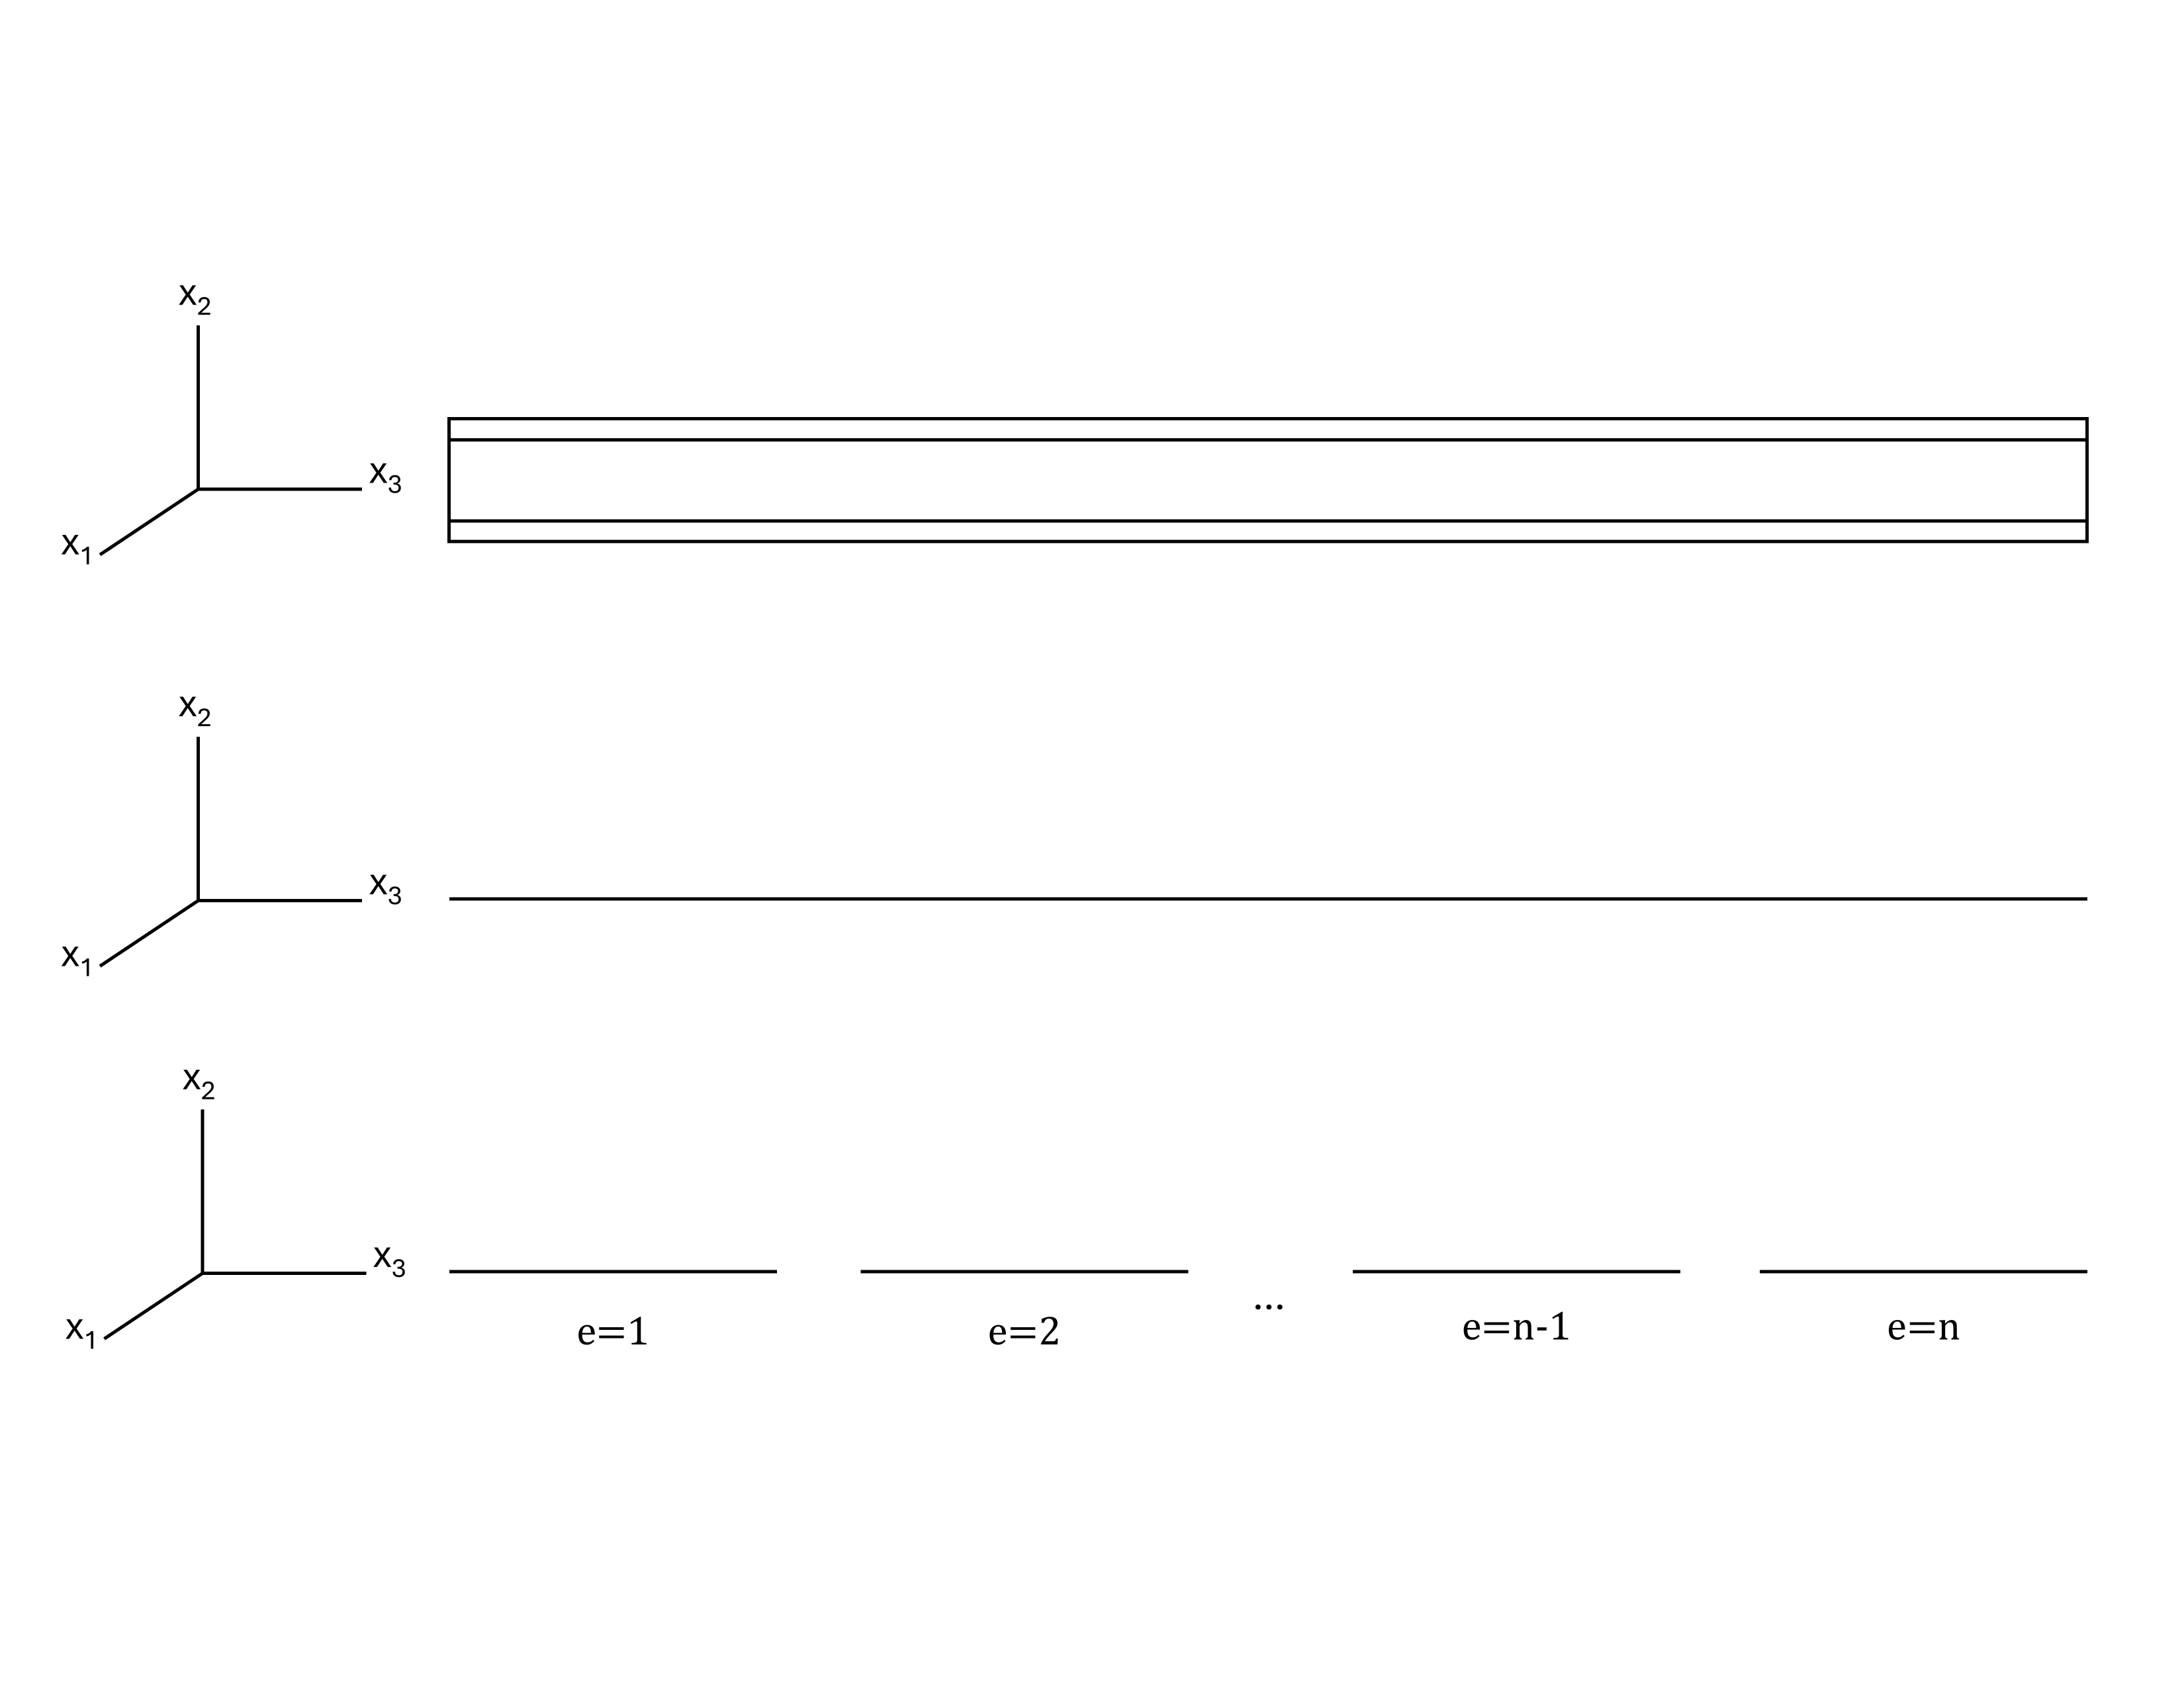
\includegraphics[width=0.7\columnwidth,trim=5.25cm 13cm 0cm 0cm, clip]{figs/beam_to_elements.png}
%}
%\centering
%\subfloat[isometric view]{
%	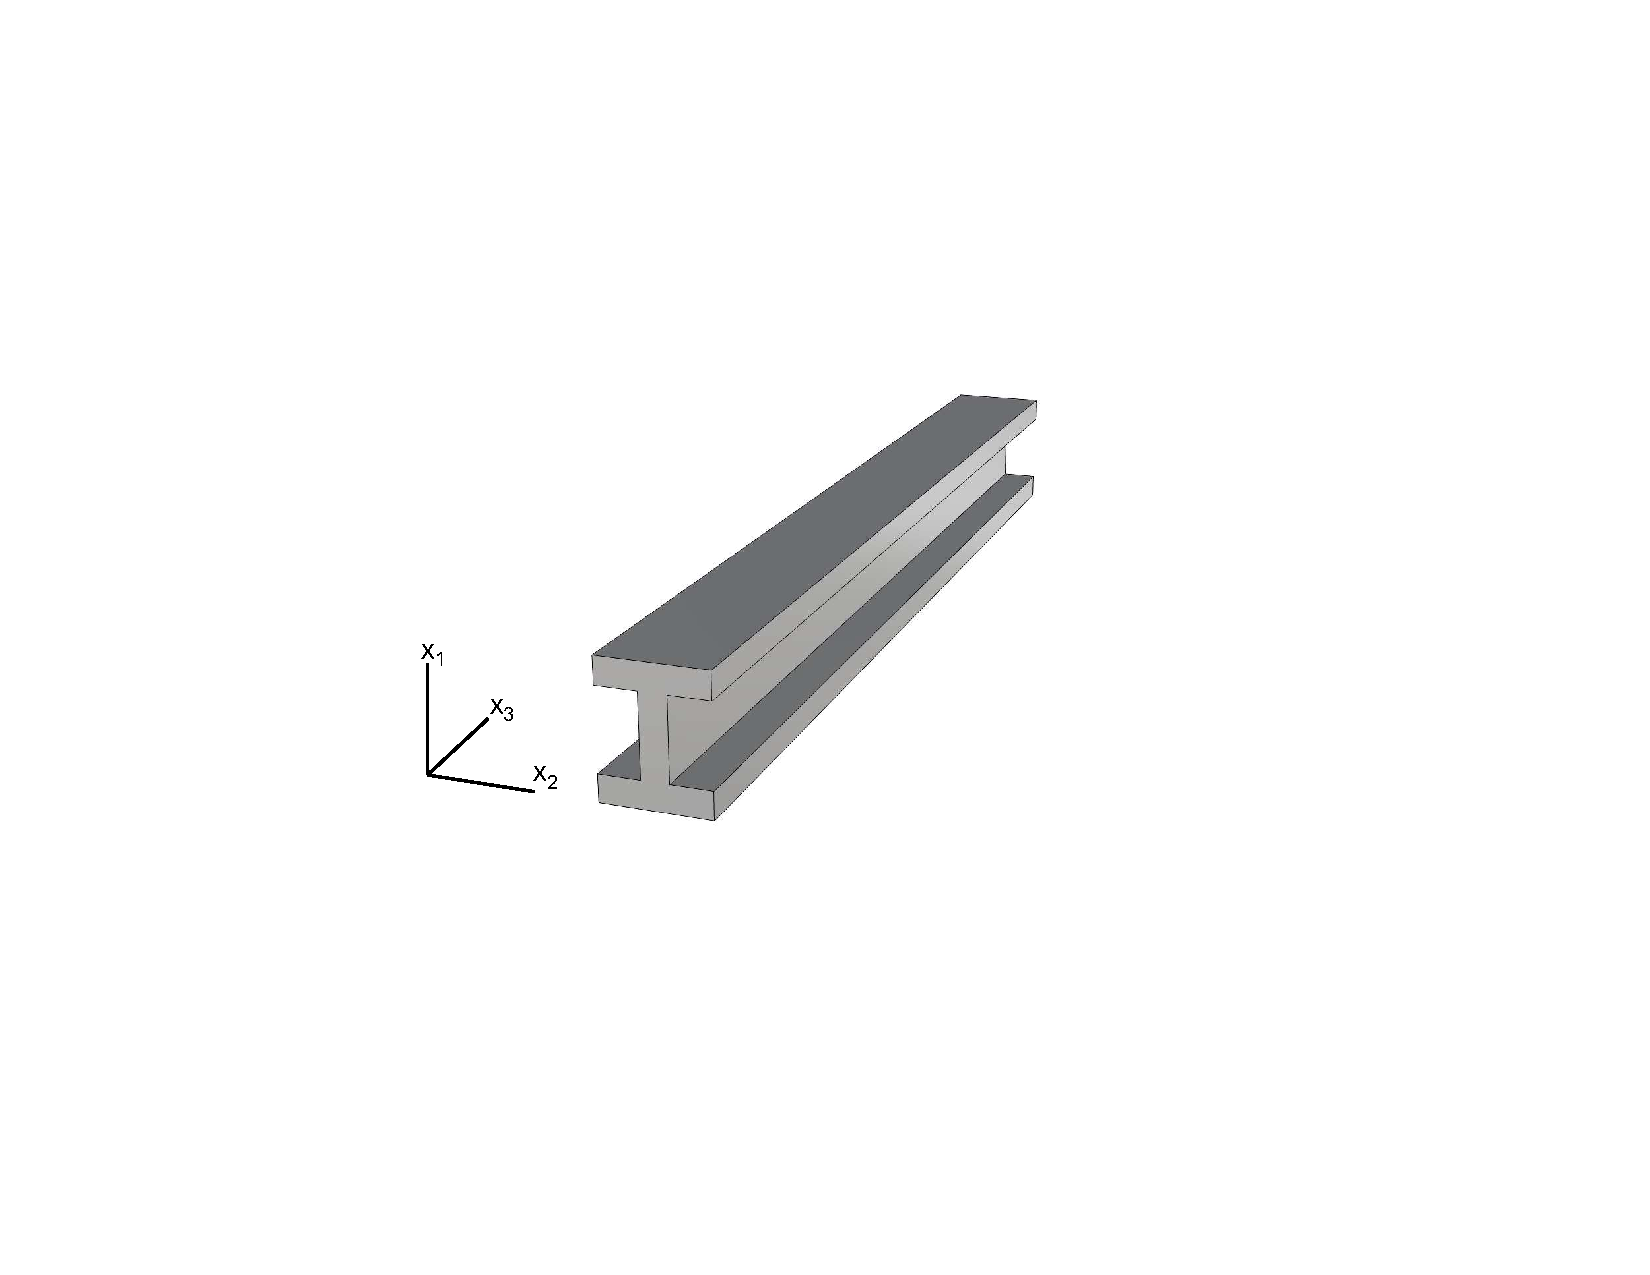
\includegraphics[width=0.25\columnwidth,trim=0cm 3cm 0cm 0cm, clip]{figs/straight.pdf}
%}
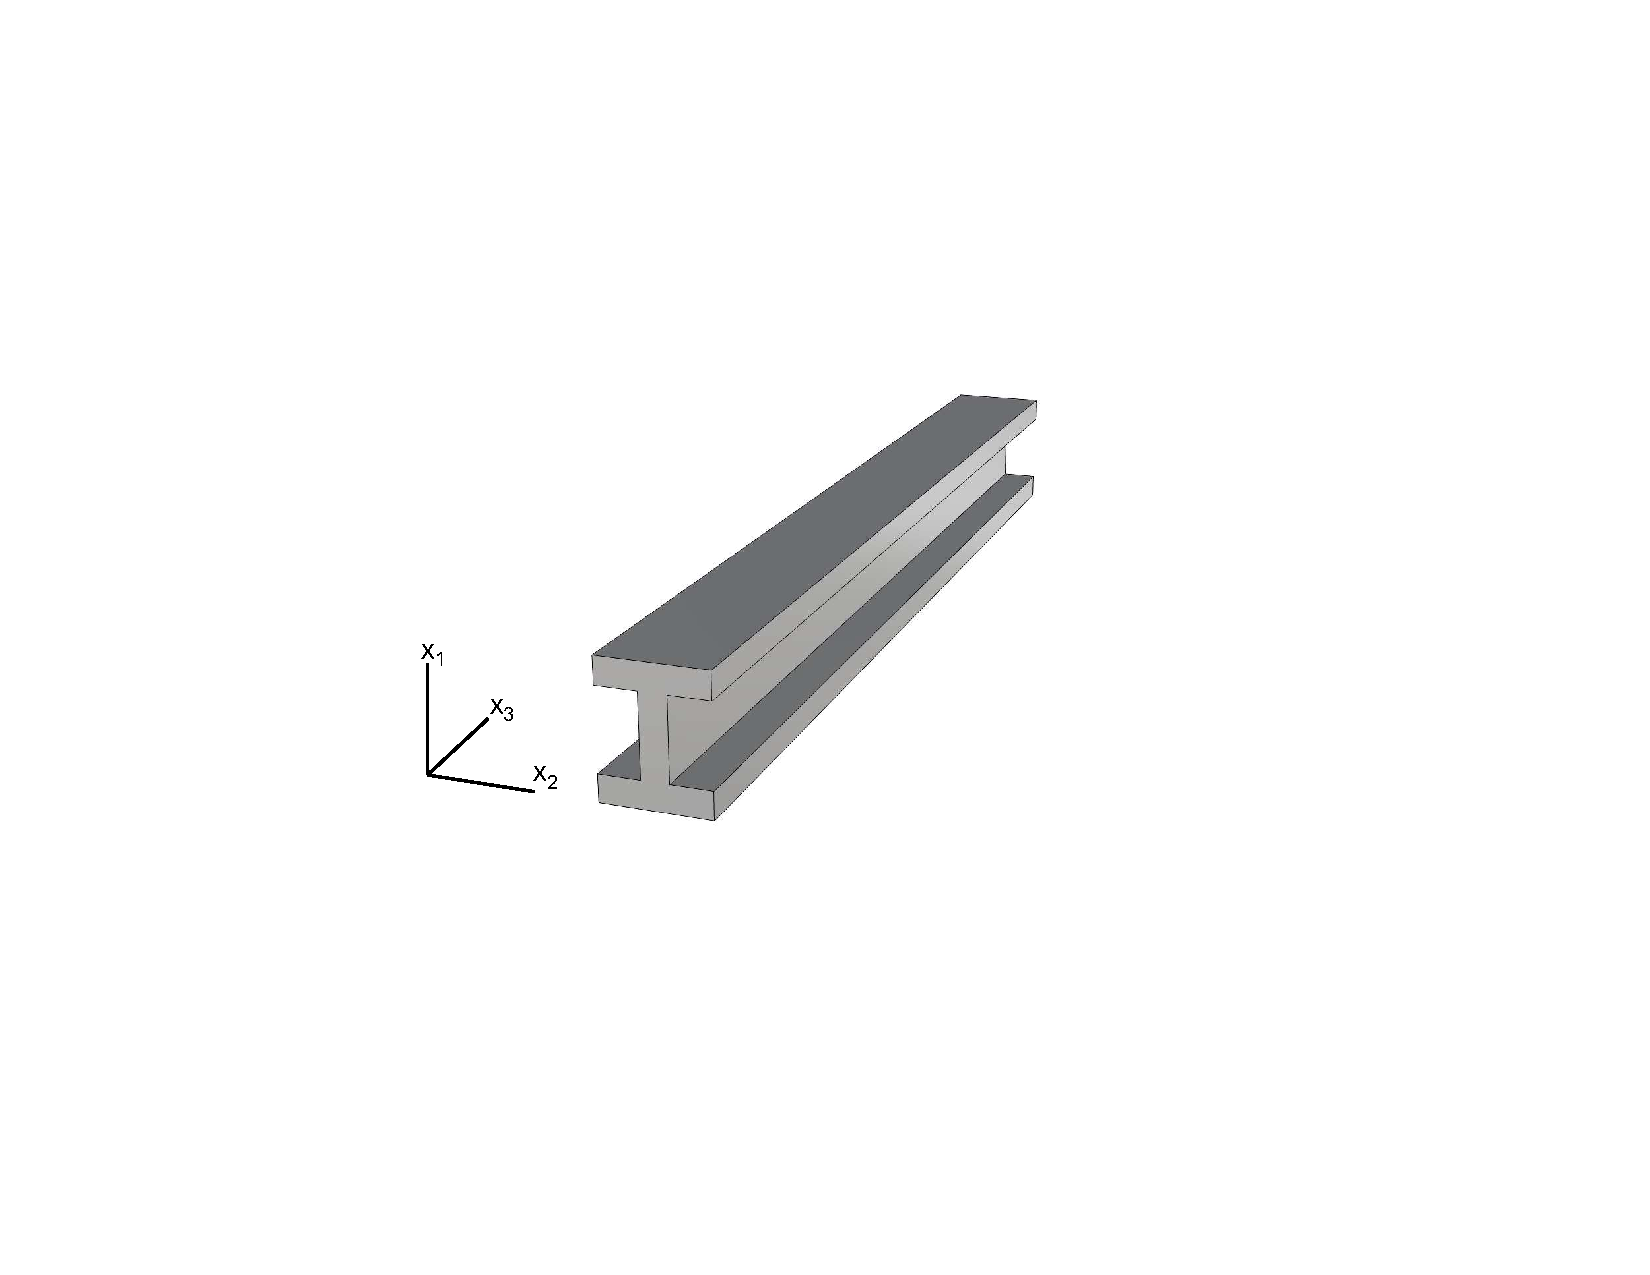
\includegraphics[width=0.95\columnwidth,trim=4cm 7cm 6cm 6.5cm, clip]{figs/straight.pdf}
\caption{The definition of the beam}
 \label{fig:beam_definition}
\end{figure}


\begin{figure}
\centering
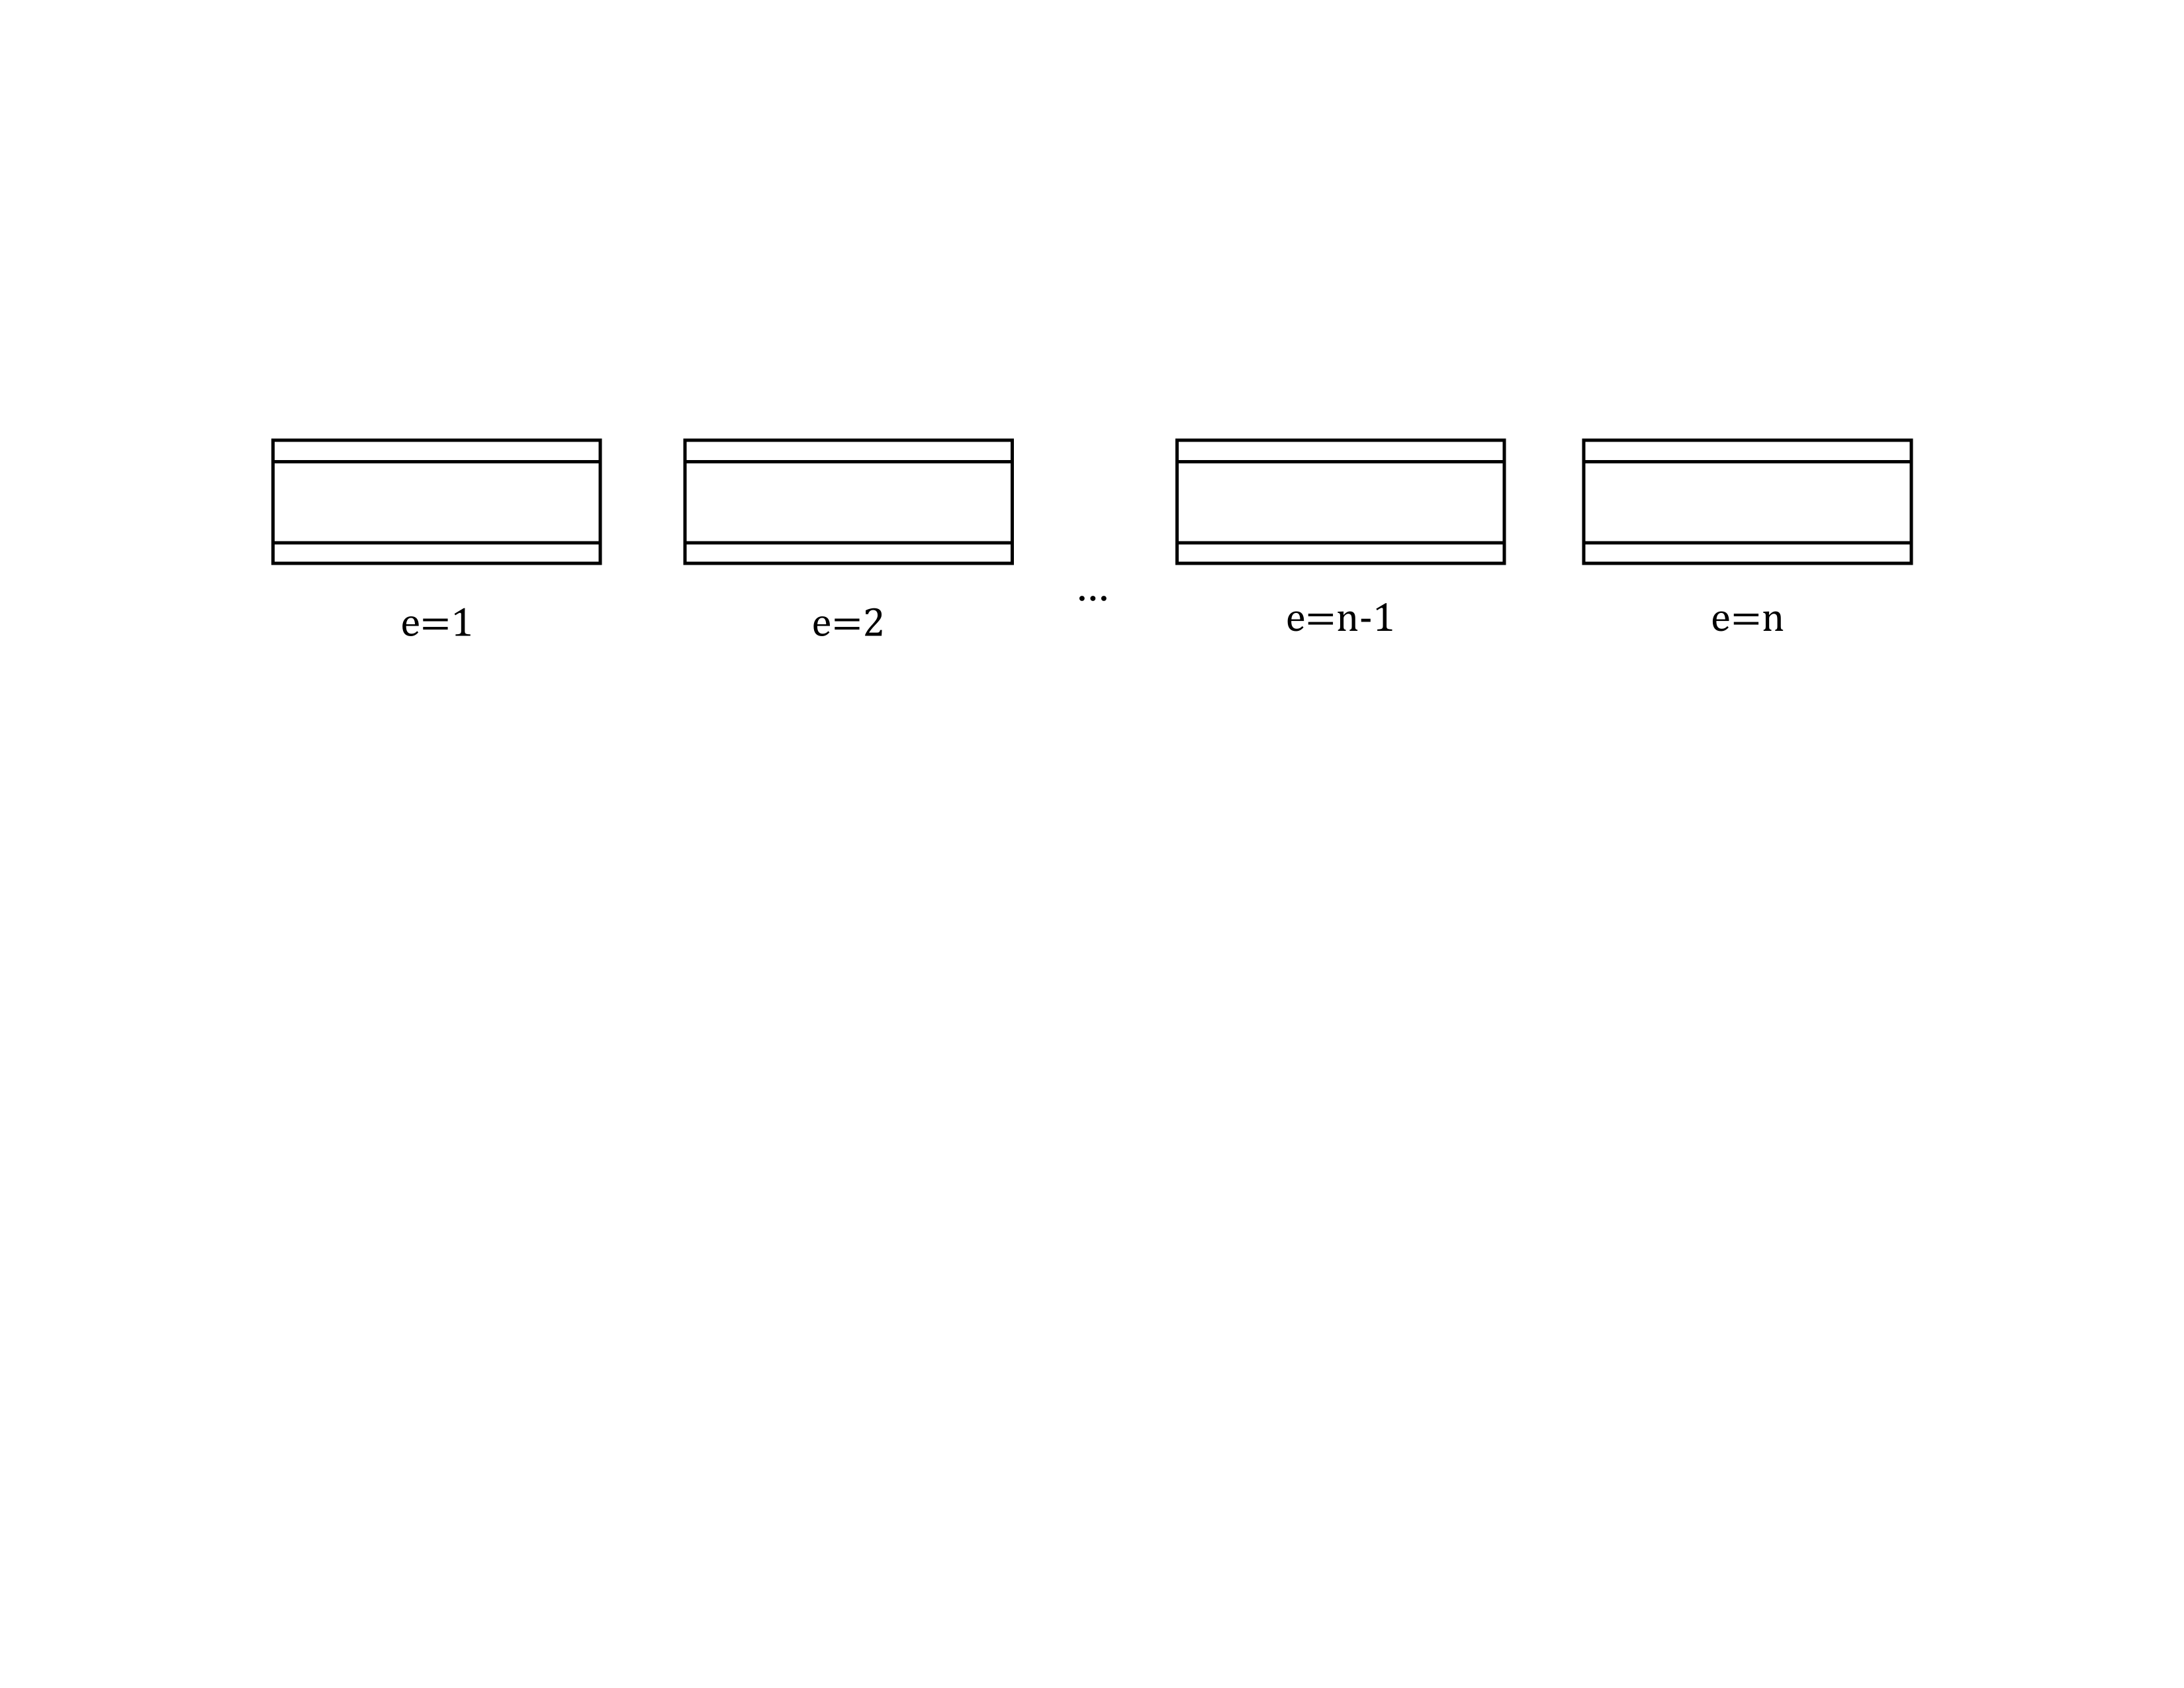
\includegraphics[width=0.7\columnwidth,trim=0cm 12cm 0cm 0cm, clip]{figs/wshape_elements.png}
\caption{The beam subdivided into n elements}
\label{fig:subdivision}
\end{figure}

\begin{figure}[htb]
\centering
\subfloat[side view]{
	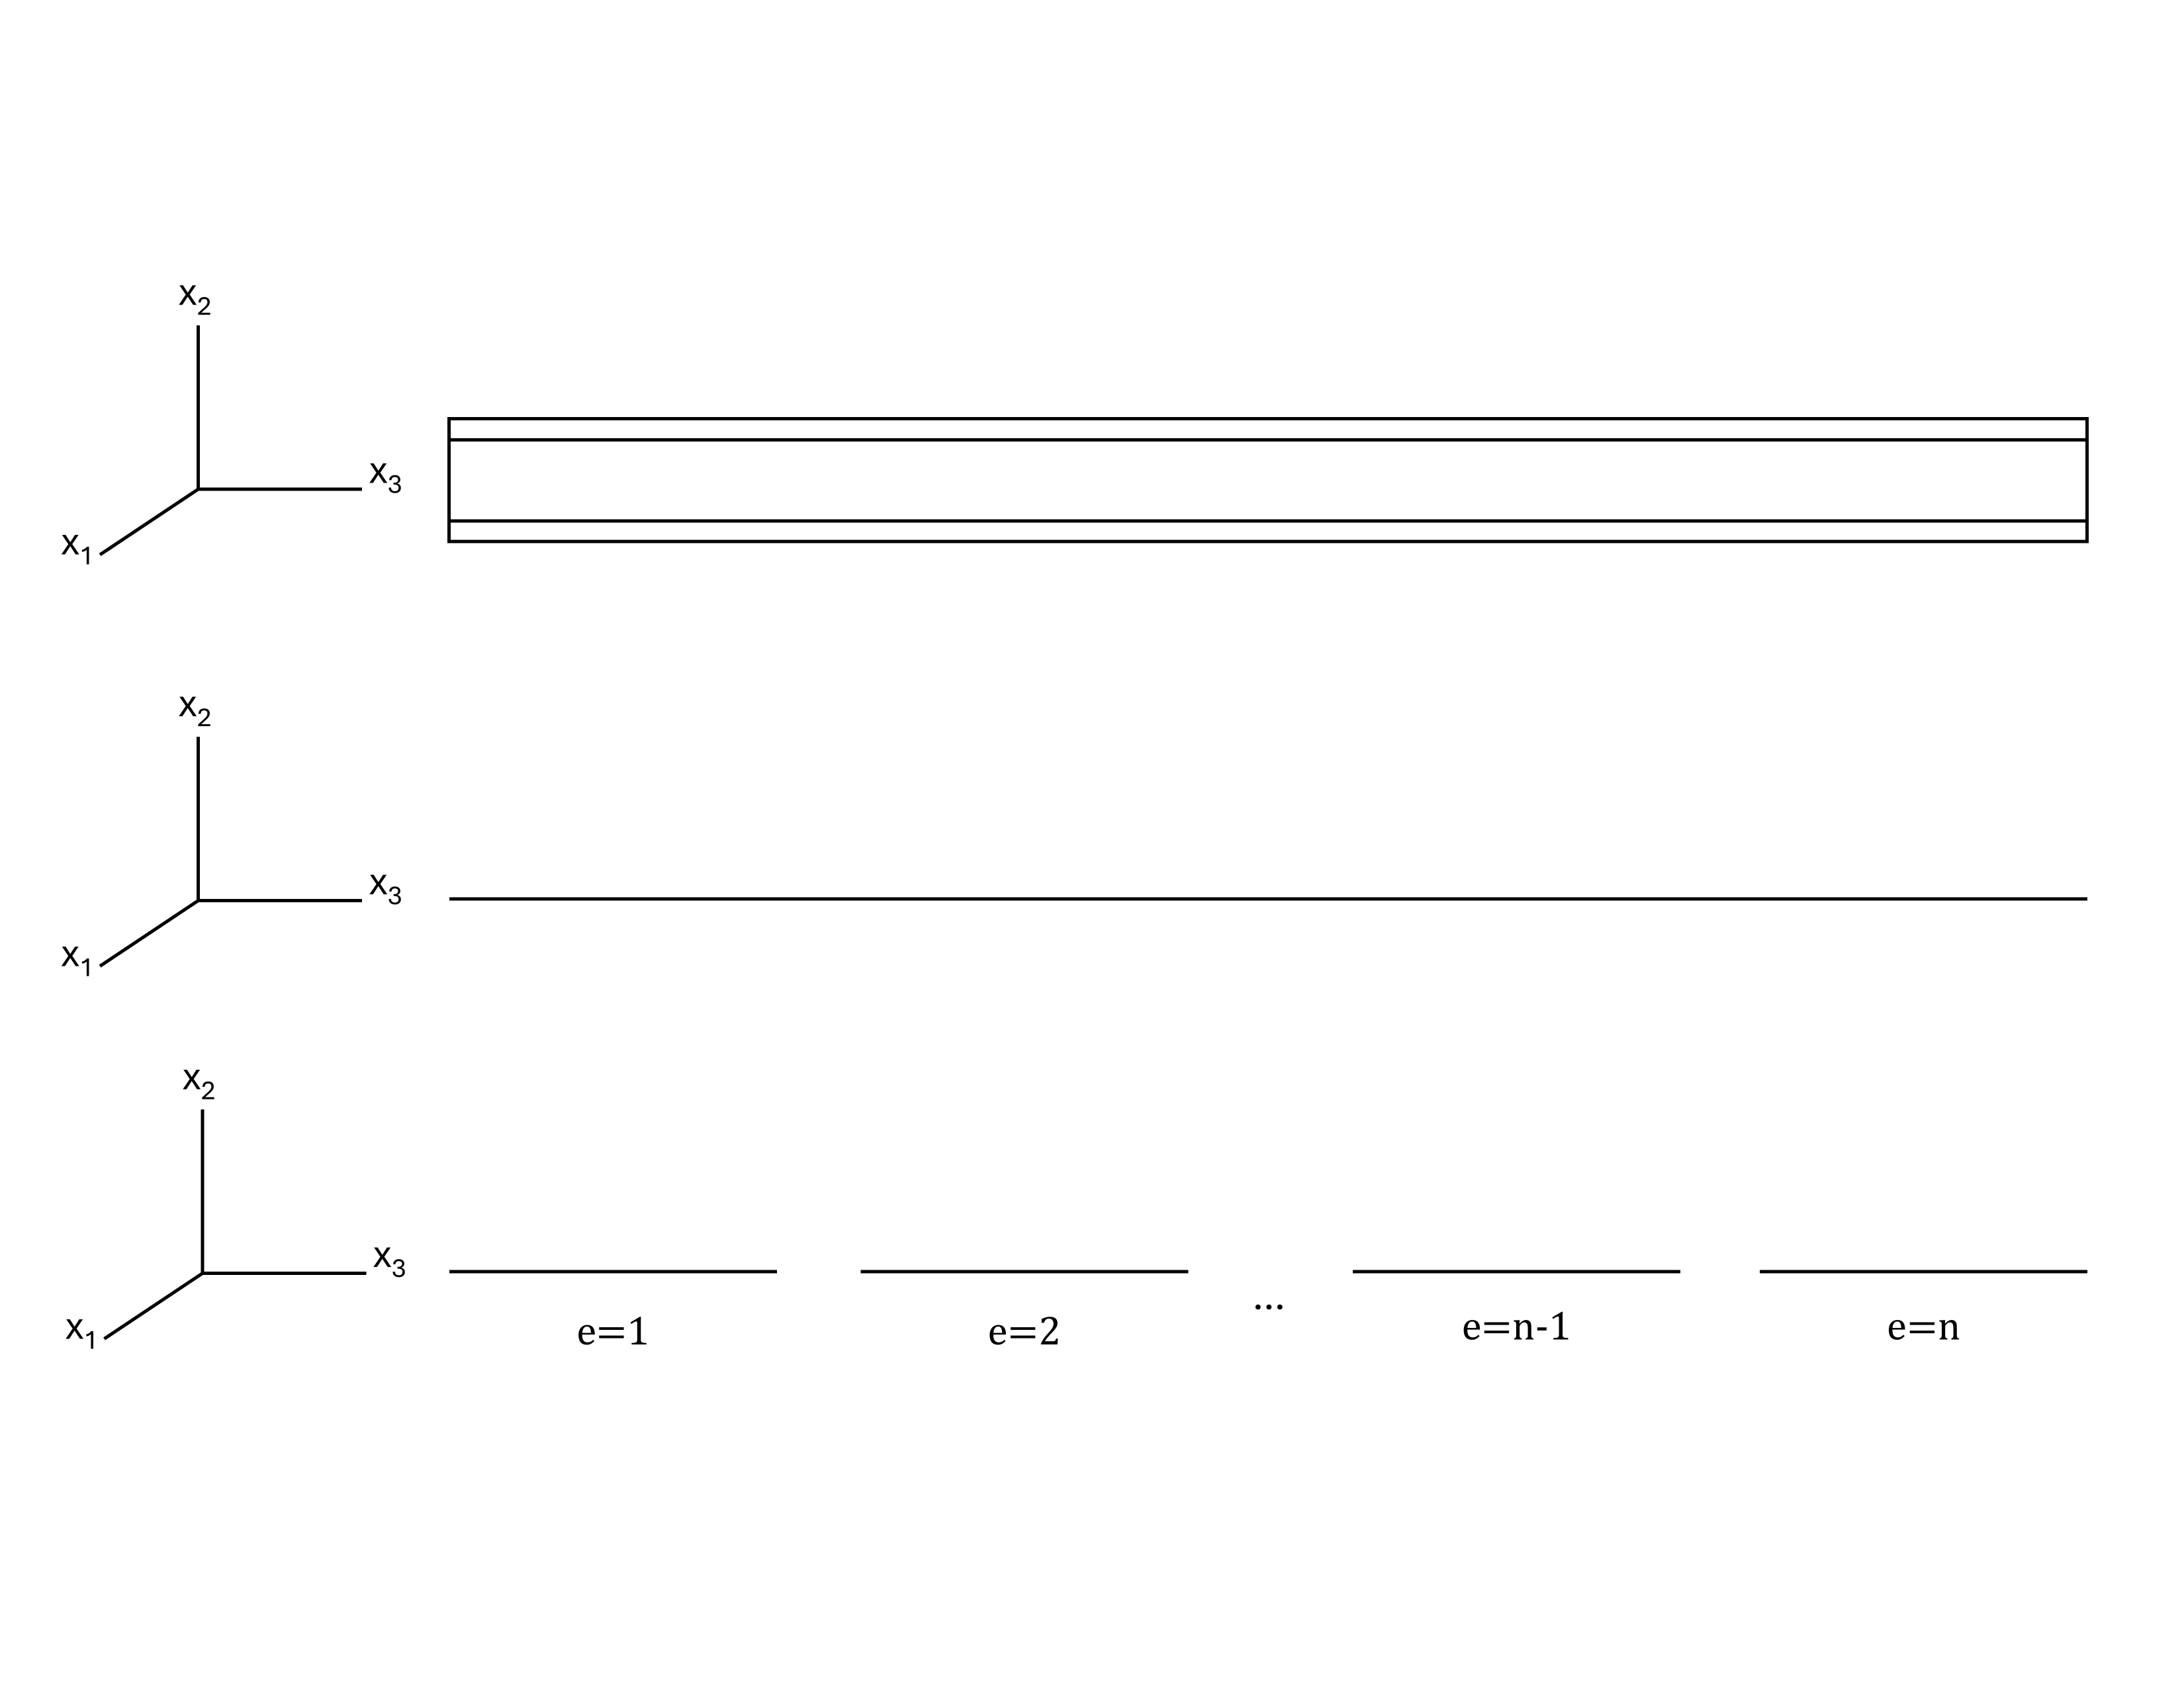
\includegraphics[width=0.7\columnwidth,trim=0cm 13cm 0cm 0cm, clip]{figs/beam_to_elements.png}
}
\centering
\subfloat[isometric view]{
	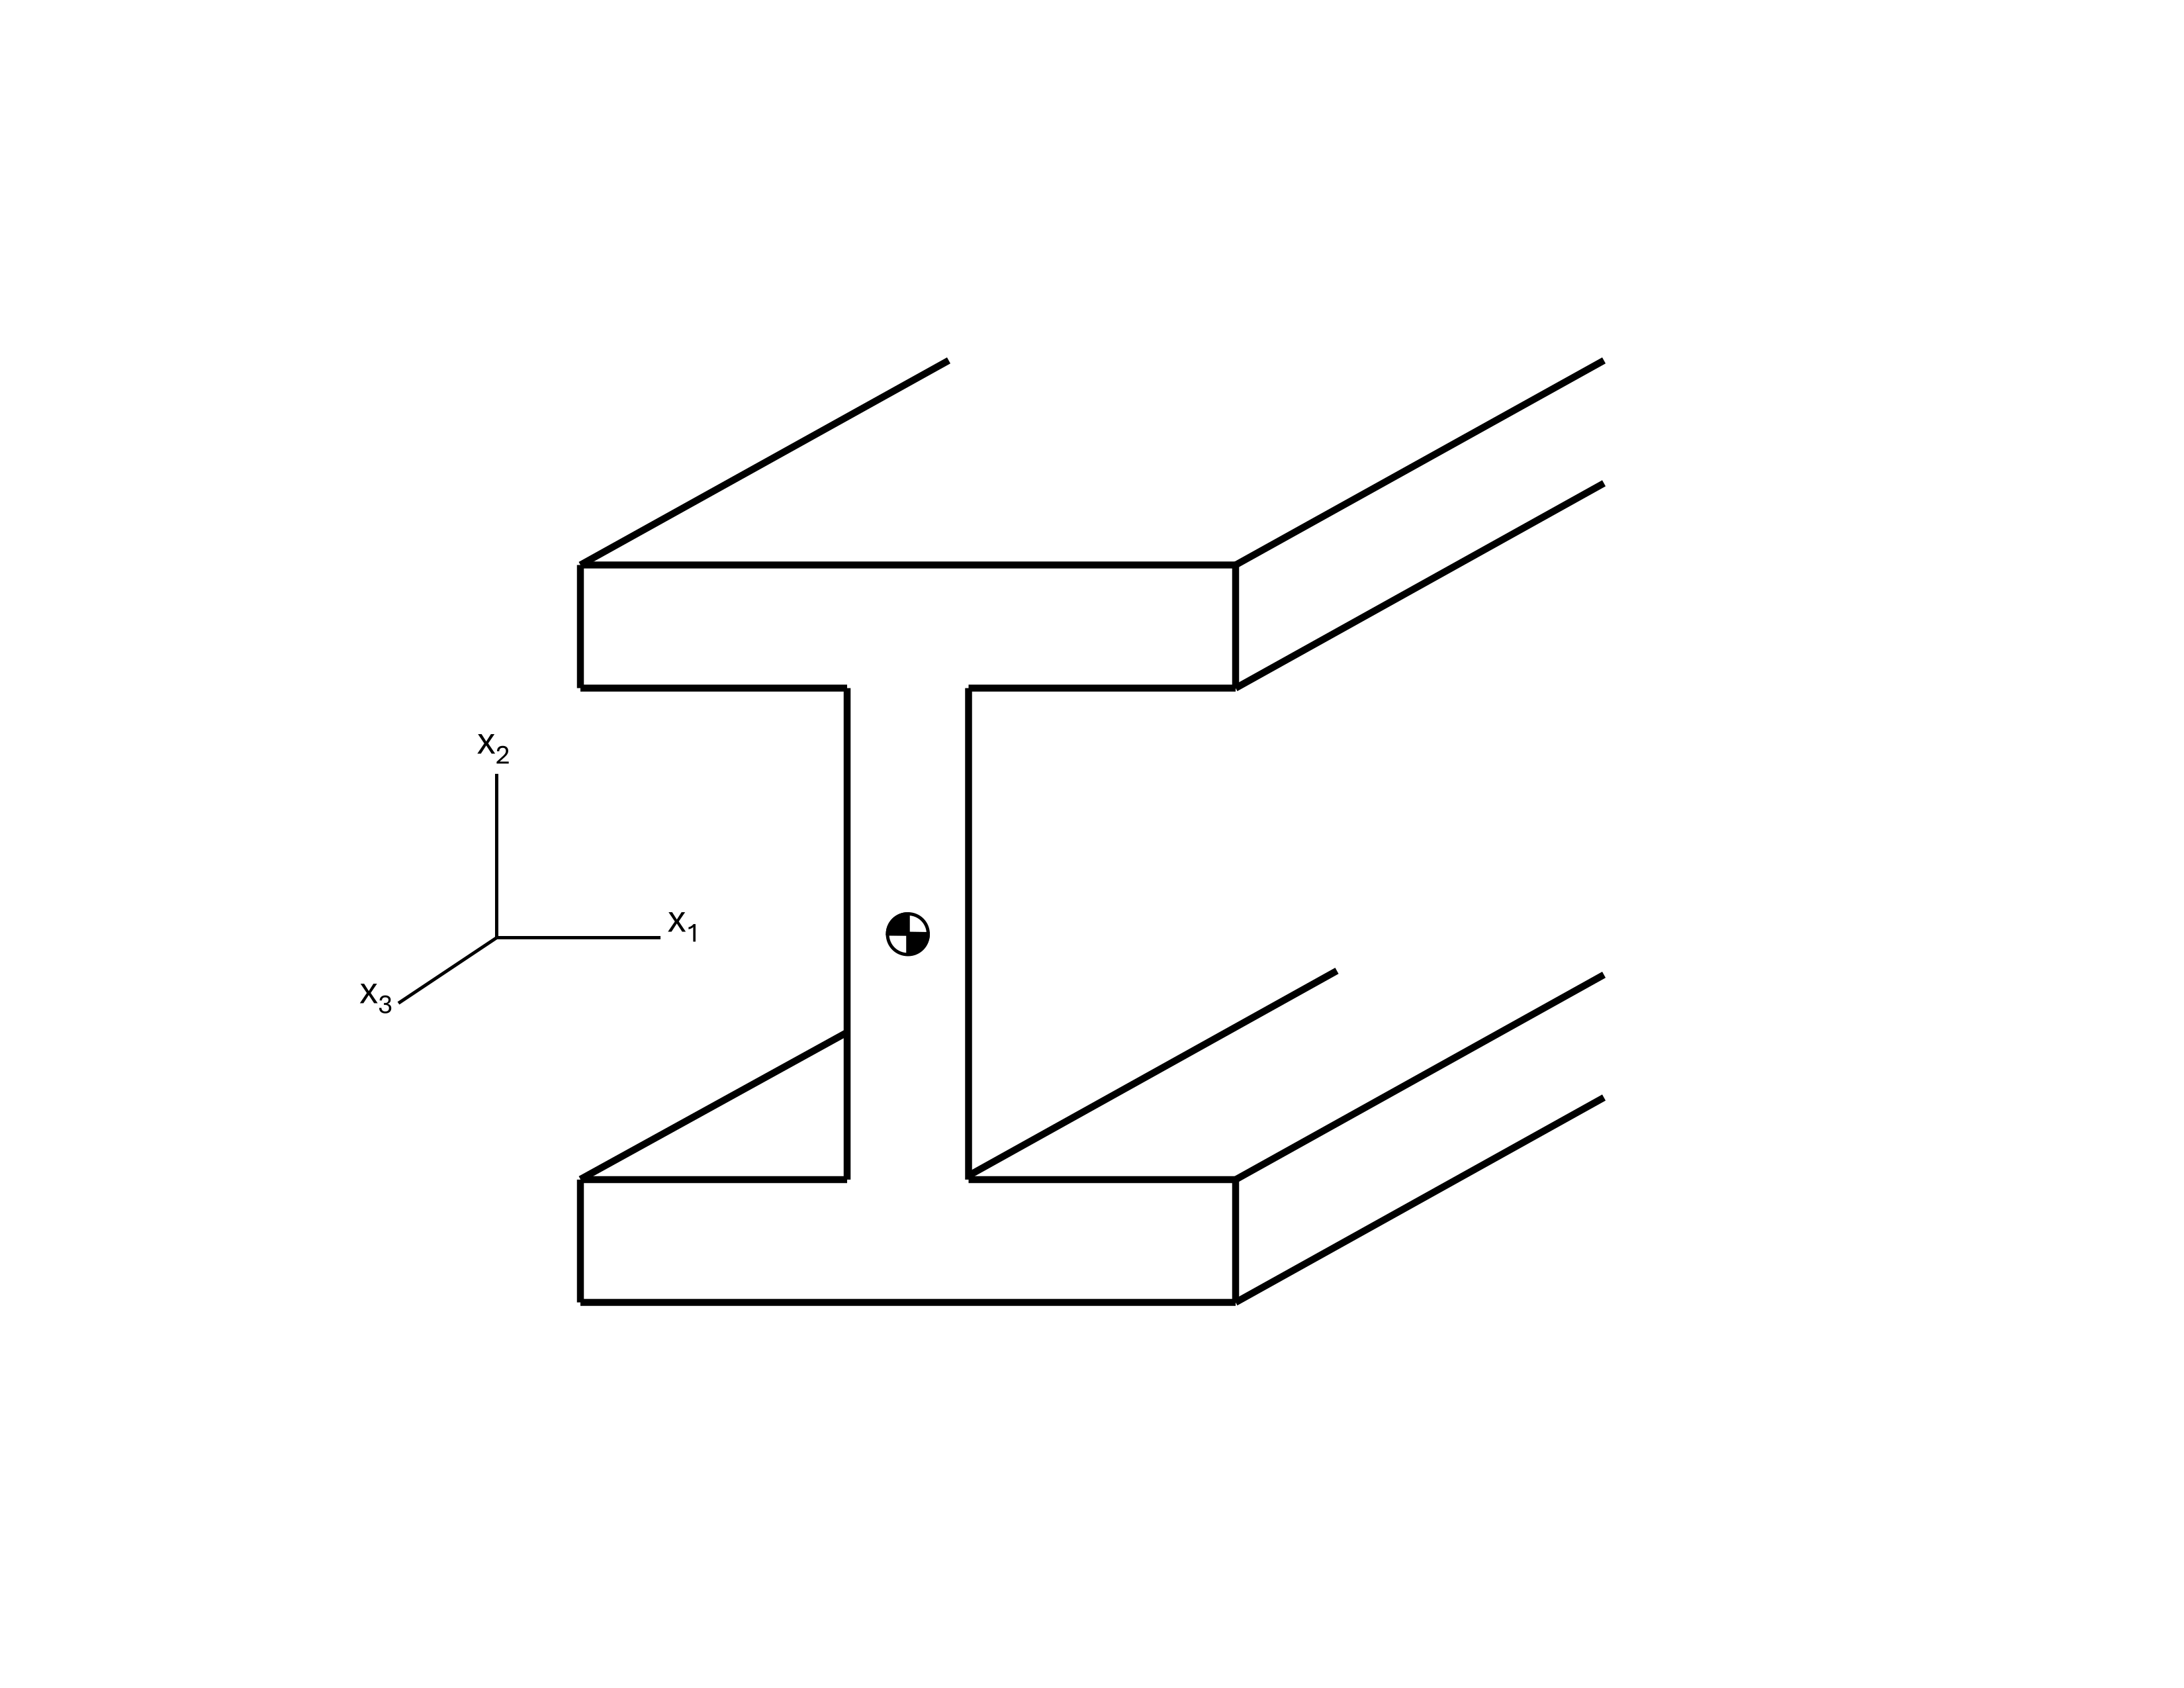
\includegraphics[width=0.25\columnwidth,trim=0cm 3cm 0cm 0cm, clip]{figs/3d_section.png}
	\label{fig:iso_view}
}
\caption{The definition of the beam}
 \label{fig:axis_definition}
\end{figure}

I will begin by outlining the assumptions made.

\paragraph{Approximating the Beam}
 We will first define a beam as our domain of interest.
The beam is displayed in \cref{fig:beam_definition}.
The domain of our beam is to first be divided into multiple sections, as shown in \cref{eq:subdivision} and \cref{fig:subdivision}, where 
$\Omega$ is the beam,
$\Omega^e$  is the $e$th element of the beam, and
$\overset{n}{\underset{e=1}{\cup}}$ is the union from element 1 to n.

\begin{equation}
 \Omega = \overset{n}{\underset{e=1}{\cup}} \Omega^e
 \label{eq:subdivision}
 \end{equation}


Thus \cref{eq:subdivision} states that the domain of interest is to be composed of beam elements numbered from 1 to n.
Furthermore, each element has local axes defined with respect to the principal axes as shown in \cref{eq:axis_definition,fig:axis_definition}, where $h^e$ is the length of each element and $A^e$ is the cross sectional area of each element.

\begin{equation}
\Omega^e = \{
(x_1^e, x_2^e, x_3^e)
|x_3^e 
\in 
[0,h^e], 
(x_1^e, x_2^2) 
\in
A^e 
\subset
\mathbb{R}^2 
\}
\label{eq:axis_definition}
\end{equation}

Furthermore, for the analysis the beam will be considered a one dimensional element. 
Thus, the beam will be approximated as a line with length $h$ that will act at the centroid of the beam as shown by the center of gravity marker in~\cref{fig:iso_view}.
In other texts, this is represented by~\cref{eq:zero_area}.

\begin{equation}
0 =
\int_{A^e} x_1^e \,dA \  =
\int_{A^e} x_2^e \,dA \ =
\int_{A^e} x_1^e x_2^e \,dA \
\label{eq:zero_area}
\end{equation}

\paragraph{Stress Tensor}
The second assummption is that $\sigma_{\alpha\beta}=0$ for $\alpha,\beta \in \{1,2\}$.
The stress tensor $\sigma$ is shown in \cref{eq:stress_tensor} and the stress element in \cref{fig:stress_element}.
By this assumption, the beam will not have normal stresses in the $x_1$ or $x_2$ directions, similar to an axial rod.
The difference between the beam and an axial rod is that it can experience shear in the $\sigma_{13}$ and $\sigma_{23}$ directions).
We know the beam will have loads applied in the $x_1$ or $x_2$ directions, which typically would mean a normal stress in those directions.
However, given our assumptions the beam will still be able to support these loads by the shear.
This assumption is made for consistency to ensure $\epsilon_{\alpha\beta} = 0$, since we are also neglecting the cross-sectional area of the beam as was shown in \cref{eq:zero_area}.
In \cref{sec:continuum_mechanics} it will be explained how we can still calculate $\epsilon_{\alpha\beta}$.

\begin{equation}
\sigma = \begin{bmatrix}
0 & 0 & \sigma_{13} \\
0 & 0 & \sigma_{23} \\
\sigma_{13} & \sigma_{23} & \sigma_{33}
\end{bmatrix}
\label{eq:stress_tensor}
\end{equation}

\begin{figure}%[htb]
\centering
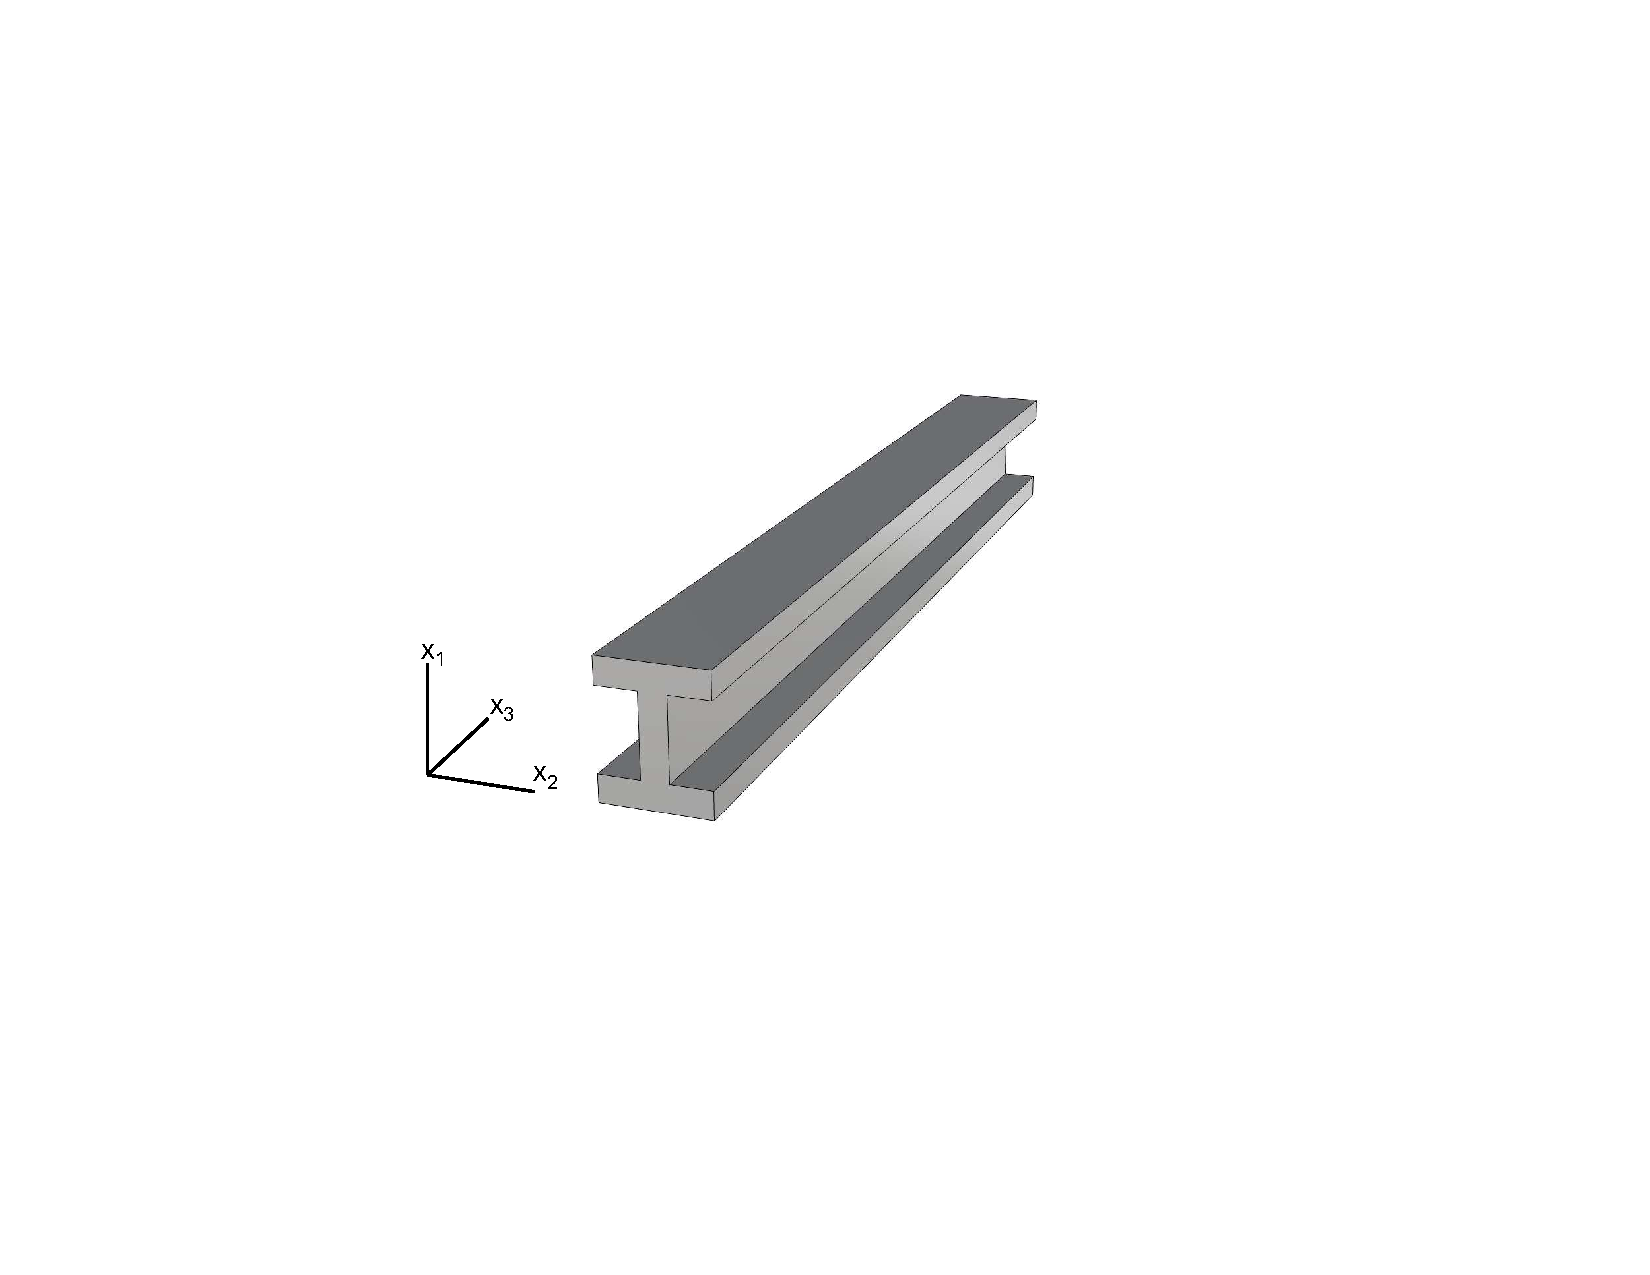
\includegraphics[width=0.95\columnwidth,trim=4cm 7cm 6cm 6.5cm, clip]{figs/straight.pdf}
\caption{The stress element of the beam in its global coordinates. CHANGE PICTURE: make a stress element with coordinate axes shown.}
\label{fig:stress_element}
\end{figure}

If we transform $\sigma$ into its principal stress form we get \cref{eq:plane_stress_tensor}.
This is significant becasue it shows that the beam is in a plane stress condition. 
A general Mohr's circle for this state of stress is shown in \cref{fig:mohrs_circle}.
This seems to justify the fact that in mechanics of materials almost all the stress tensors we worked with were simplified to the plane stress condition or similar. 

\begin{equation}
\sigma* = \begin{bmatrix}
 \frac{\sigma_{33} + \sqrt{\sigma_{33}^2 + 4(\sigma_{13}^2 + \sigma_{23}^2)}}{2} & 0 & 0 \\
0 &  \frac{\sigma_{33} - \sqrt{\sigma_{33}^2 + 4(\sigma_{13}^2 + \sigma_{23}^2)}}{2} & 0 \\
0 & 0 & 0
\end{bmatrix}
\label{eq:plane_stress_tensor}
\end{equation}

\begin{figure}
\centering
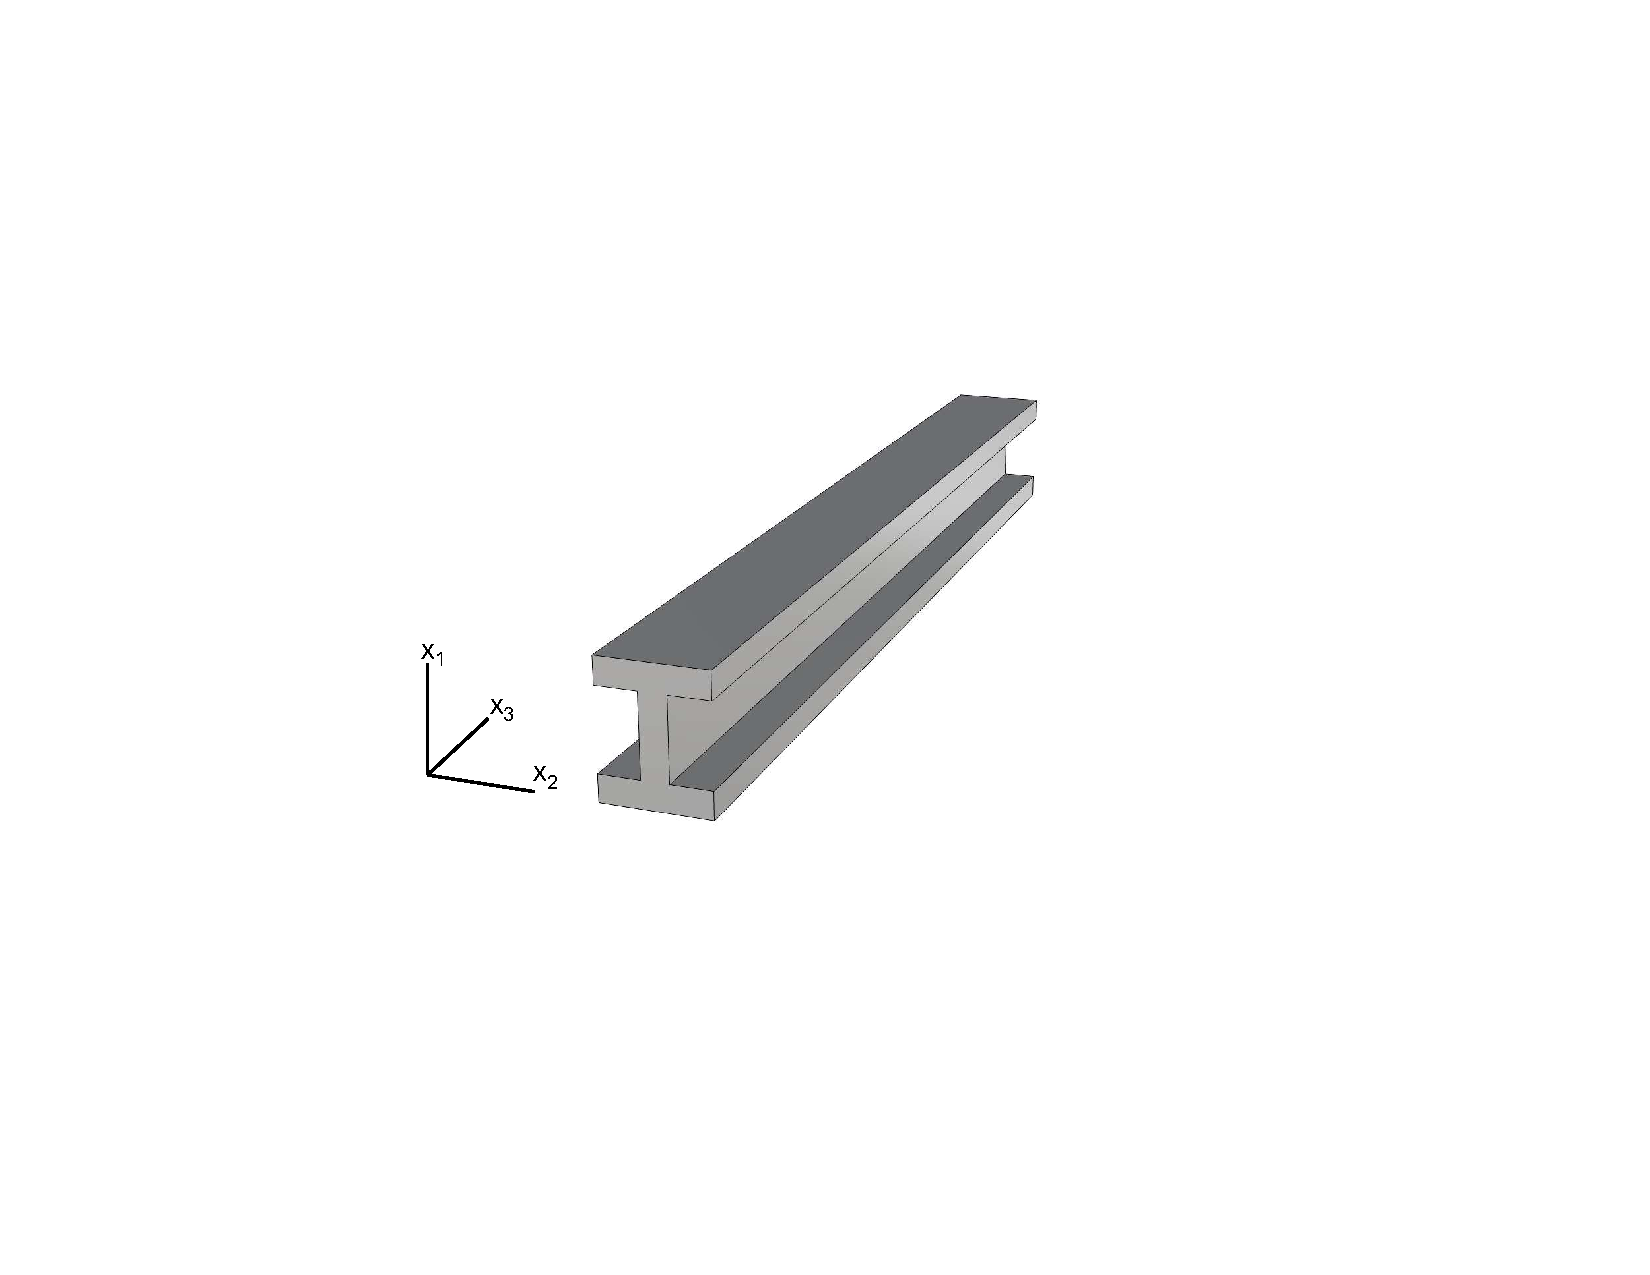
\includegraphics[width=0.95\columnwidth,trim=4cm 7cm 6cm 6.5cm, clip]{figs/straight.pdf}
\label{fig:mohrs_circle}
\caption{The generalized Mohr's circle for the plane stress condition. CHANGE PICTURE: make a Mohr's circle like the one on pg 85 (pg 25 of 61-80) in Continuum Mechanics Text}
\end{figure}

\paragraph{Displacements}
The kinematics of the beam will be accounted for using \cref{eq:u1, eq:u2, eq:u3}.
The translation of the beam is represented by $w_i$, where $i$ is the direction of the translation.
The rotation of the beam is represented by $\theta_i$.
As can be observed from the equations, $w_i$ and $\theta_i$ are functions of only $x_3$, the location along the length of the beam.
That is true because the beam is collapsed to a one-dimensional element.
The overall displacement of a point on the beam is $u_i$, which acts as a function of $x_1$, $x_2$, and $x_3$.
\cref{fig:w_theta_displacements} displays a positive displacement in each coordinate direction for both translations and rotations. 

\begin{equation}
u_1(x_1, x_2, x_3)=w_1(x_3)-x_2\theta_3(x_3)
\label{eq:u1}
\end{equation}

\begin{equation}
u_2(x_1, x_2, x_3)=w_2(x_3)+x_1\theta_3(x_3)
\label{eq:u2}
\end{equation}

\begin{equation}
u_3(x_1, x_2, x_3)=w_3(x_3)-x_1\theta_2(x_3)+x_2\theta_1(x_3)
\label{eq:u3}
\end{equation}

\begin{figure}
\centering
\subfloat[No displacement]{
	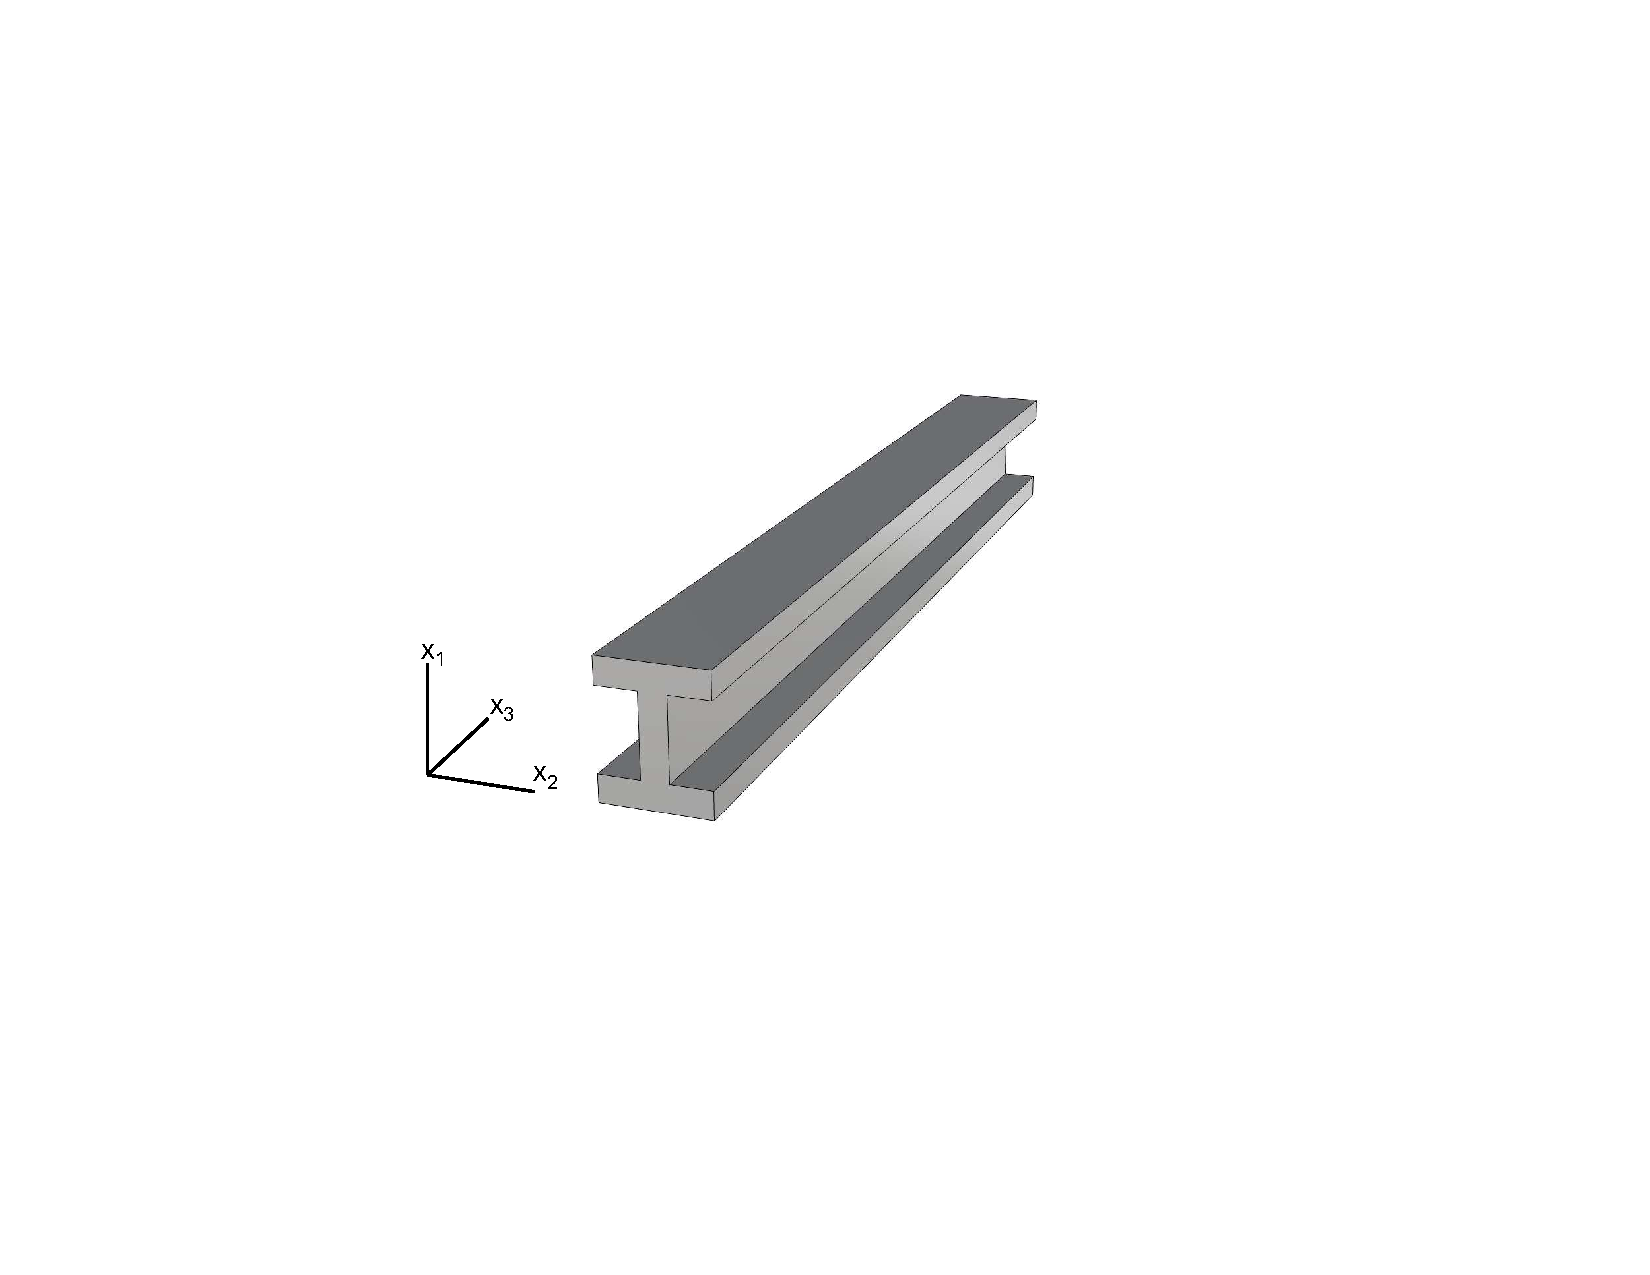
\includegraphics[width=0.2\columnwidth,trim=4cm 7cm 6cm 6.5cm, clip]{figs/straight.pdf}
}
\\
\subfloat[$w_1$]{
	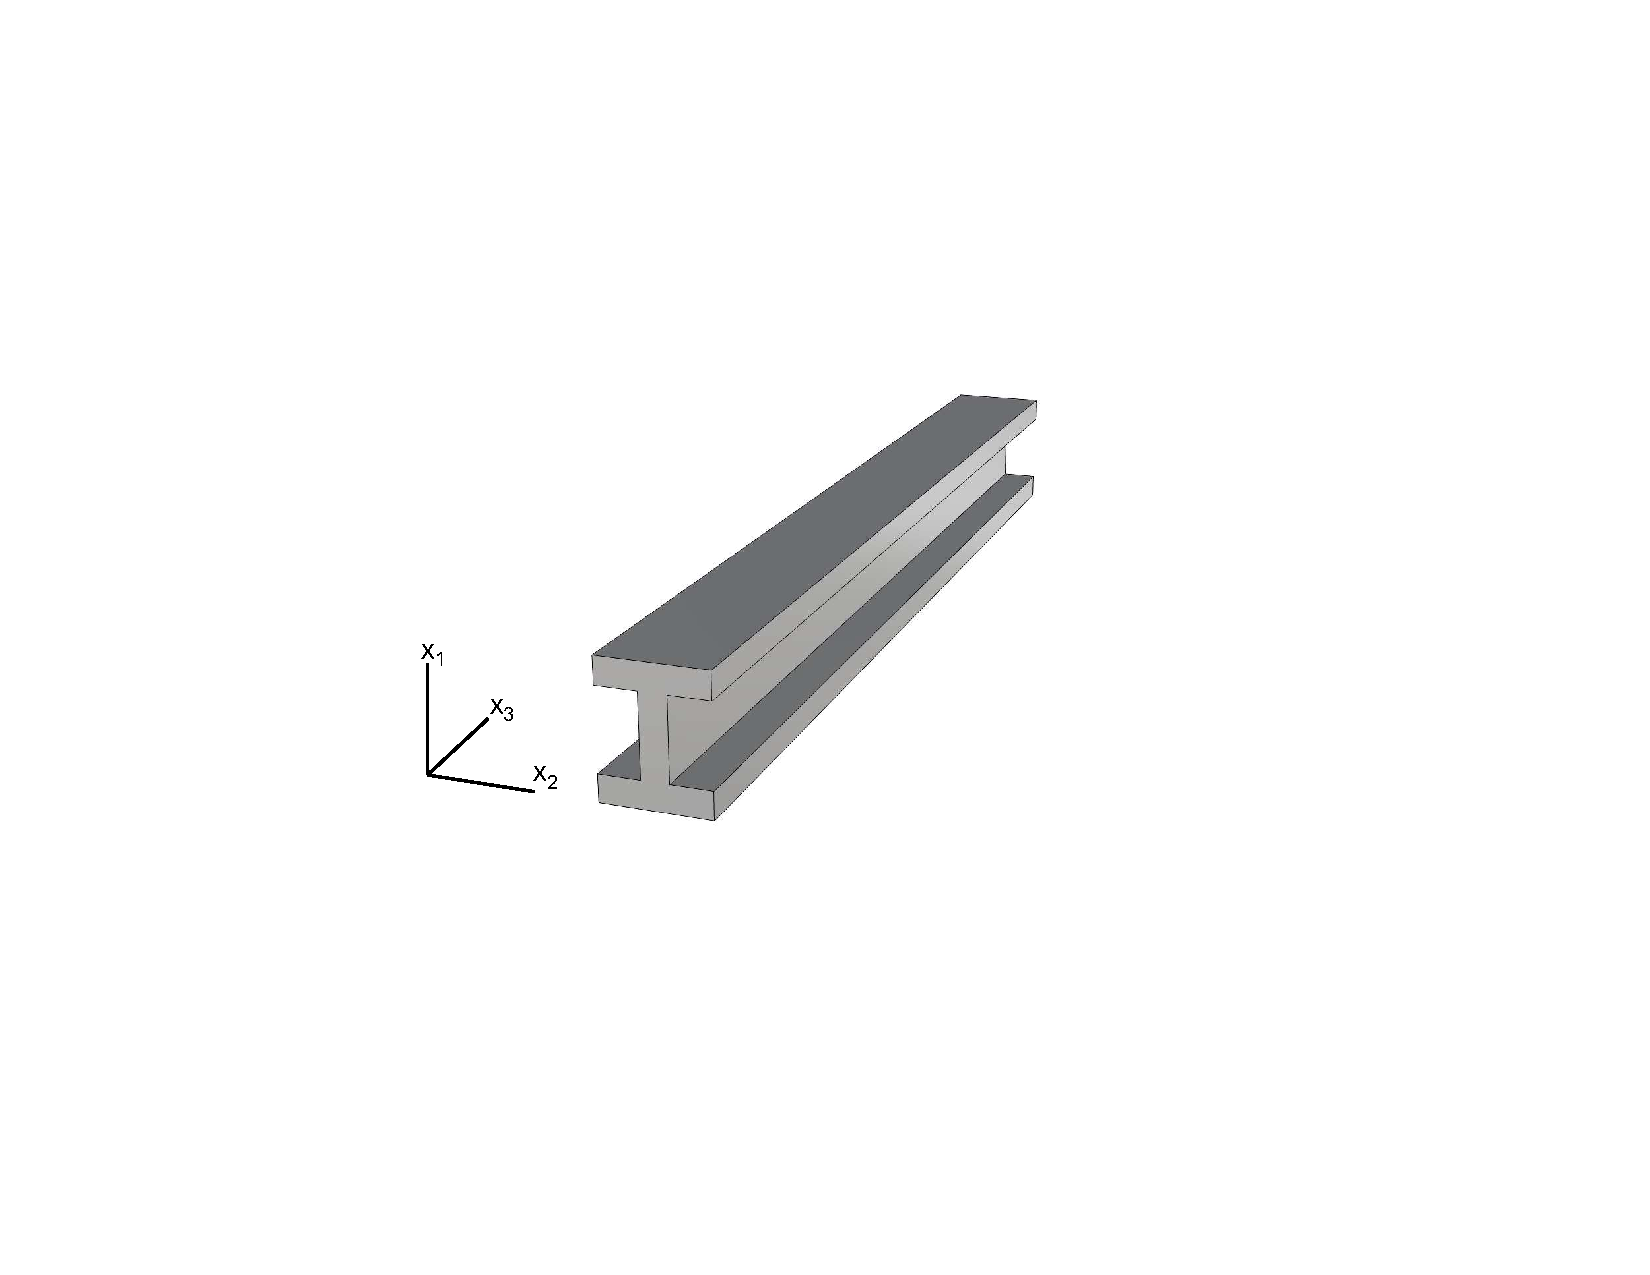
\includegraphics[width=0.2\columnwidth,trim=4cm 7cm 6cm 6.5cm, clip]{figs/straight.pdf}
}
\subfloat[$w_2$]{
	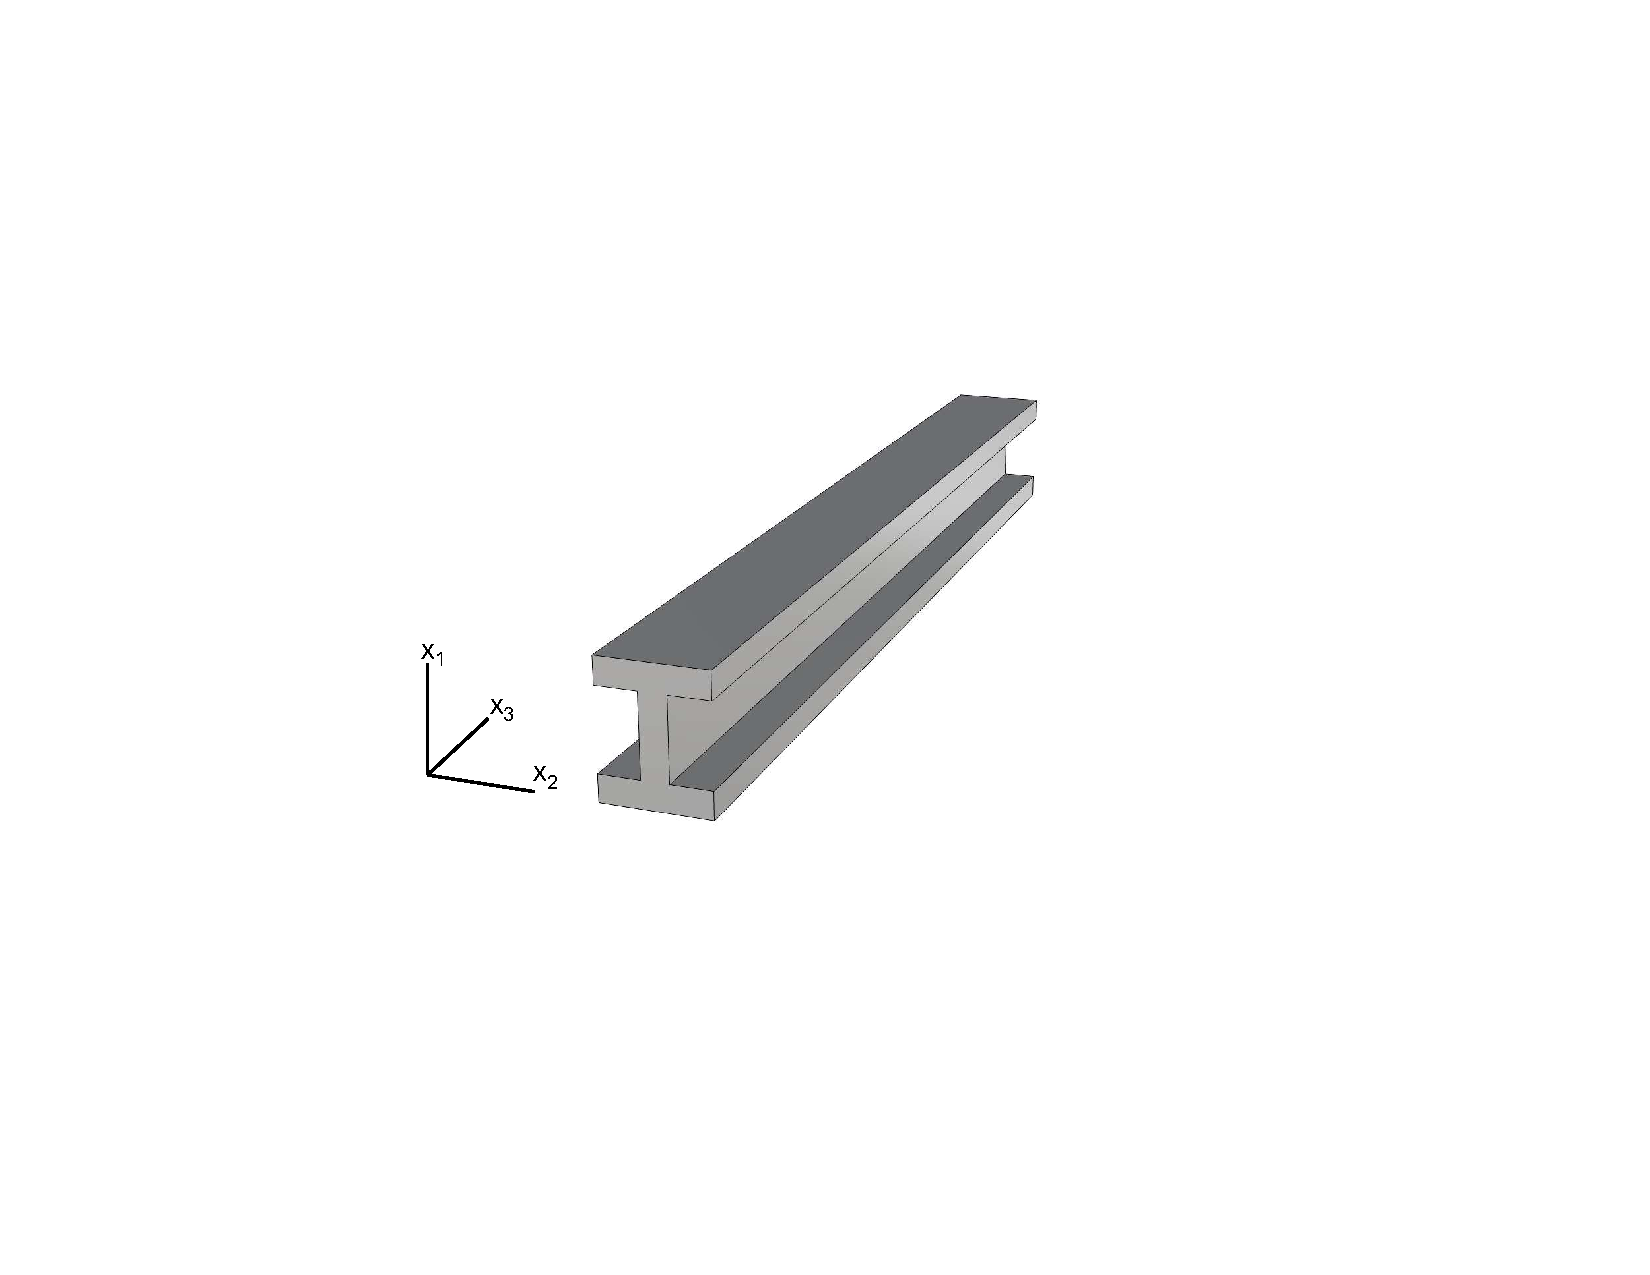
\includegraphics[width=0.2\columnwidth,trim=4cm 7cm 6cm 6.5cm, clip]{figs/straight.pdf}
}
\subfloat[$w_3$]{
	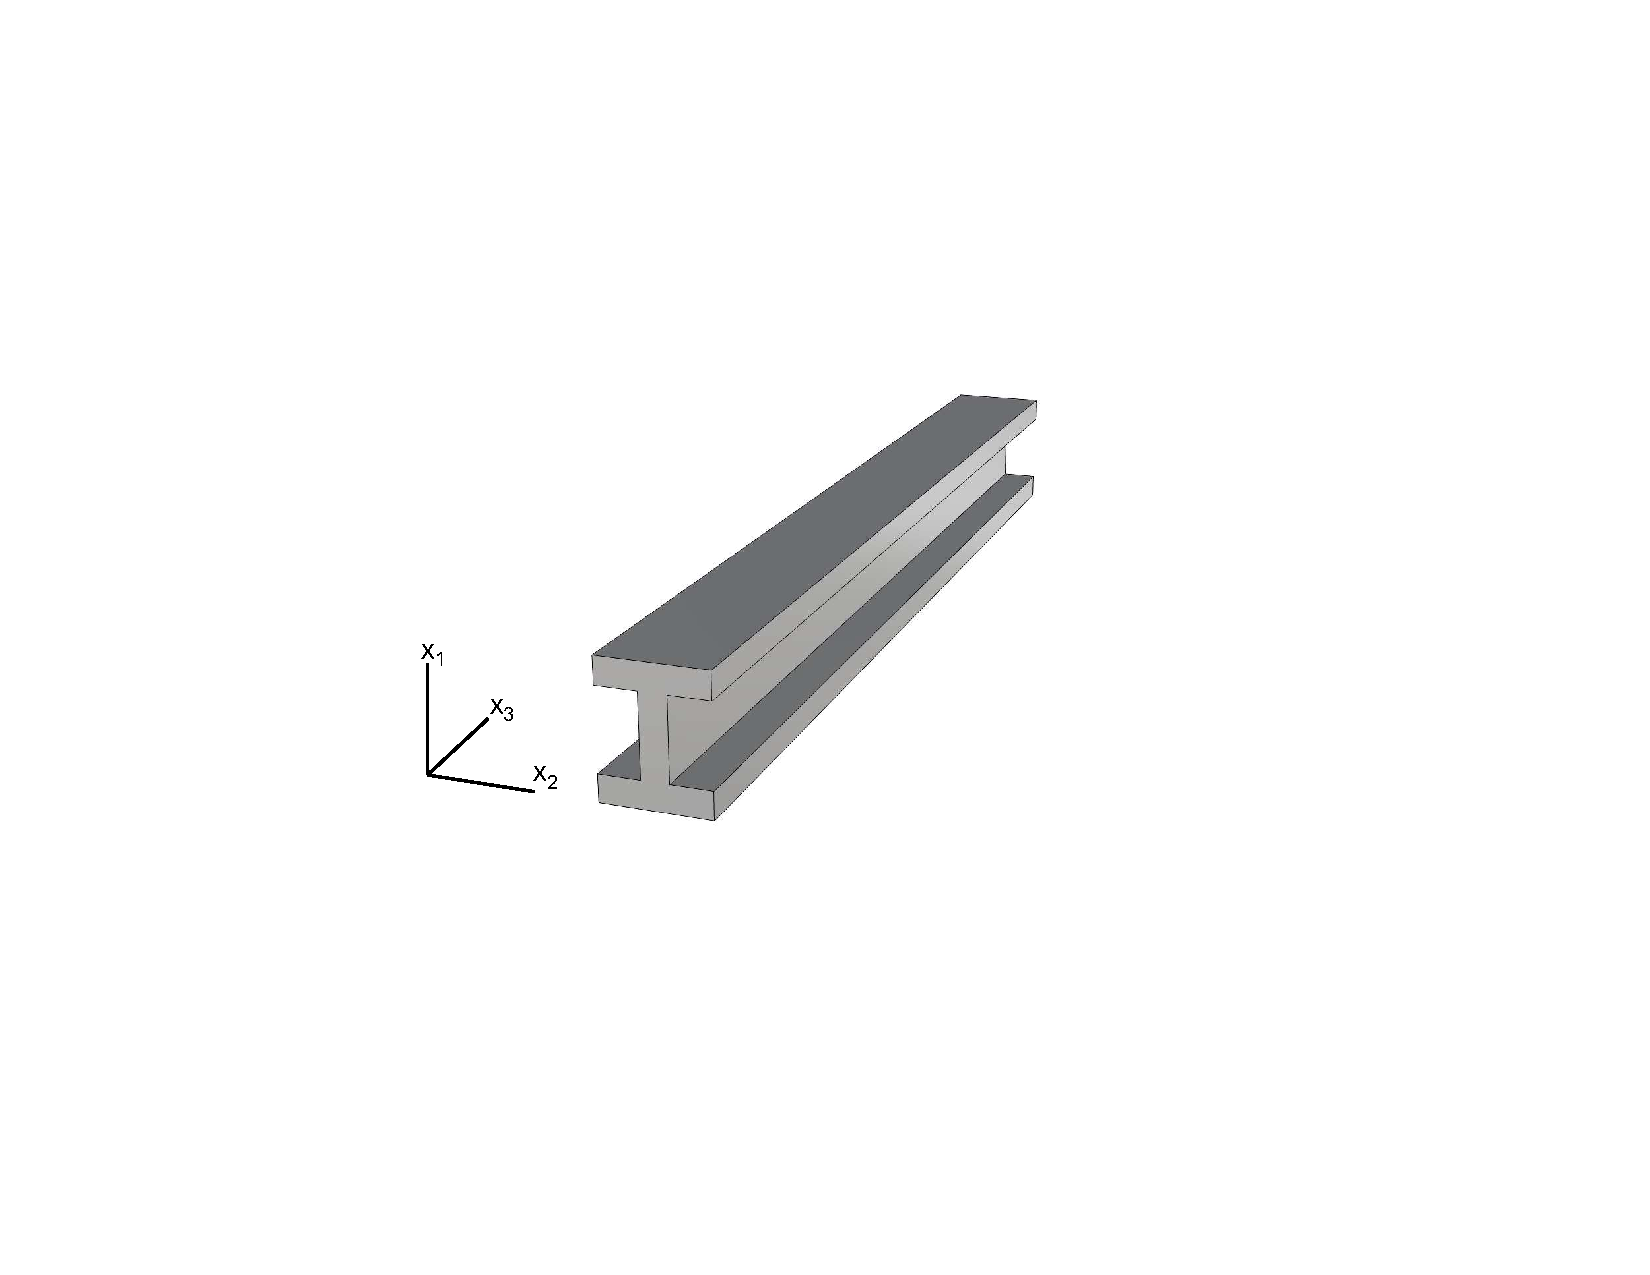
\includegraphics[width=0.2\columnwidth,trim=4cm 7cm 6cm 6.5cm, clip]{figs/straight.pdf}
}
\\
\subfloat[$\theta_1$]{
	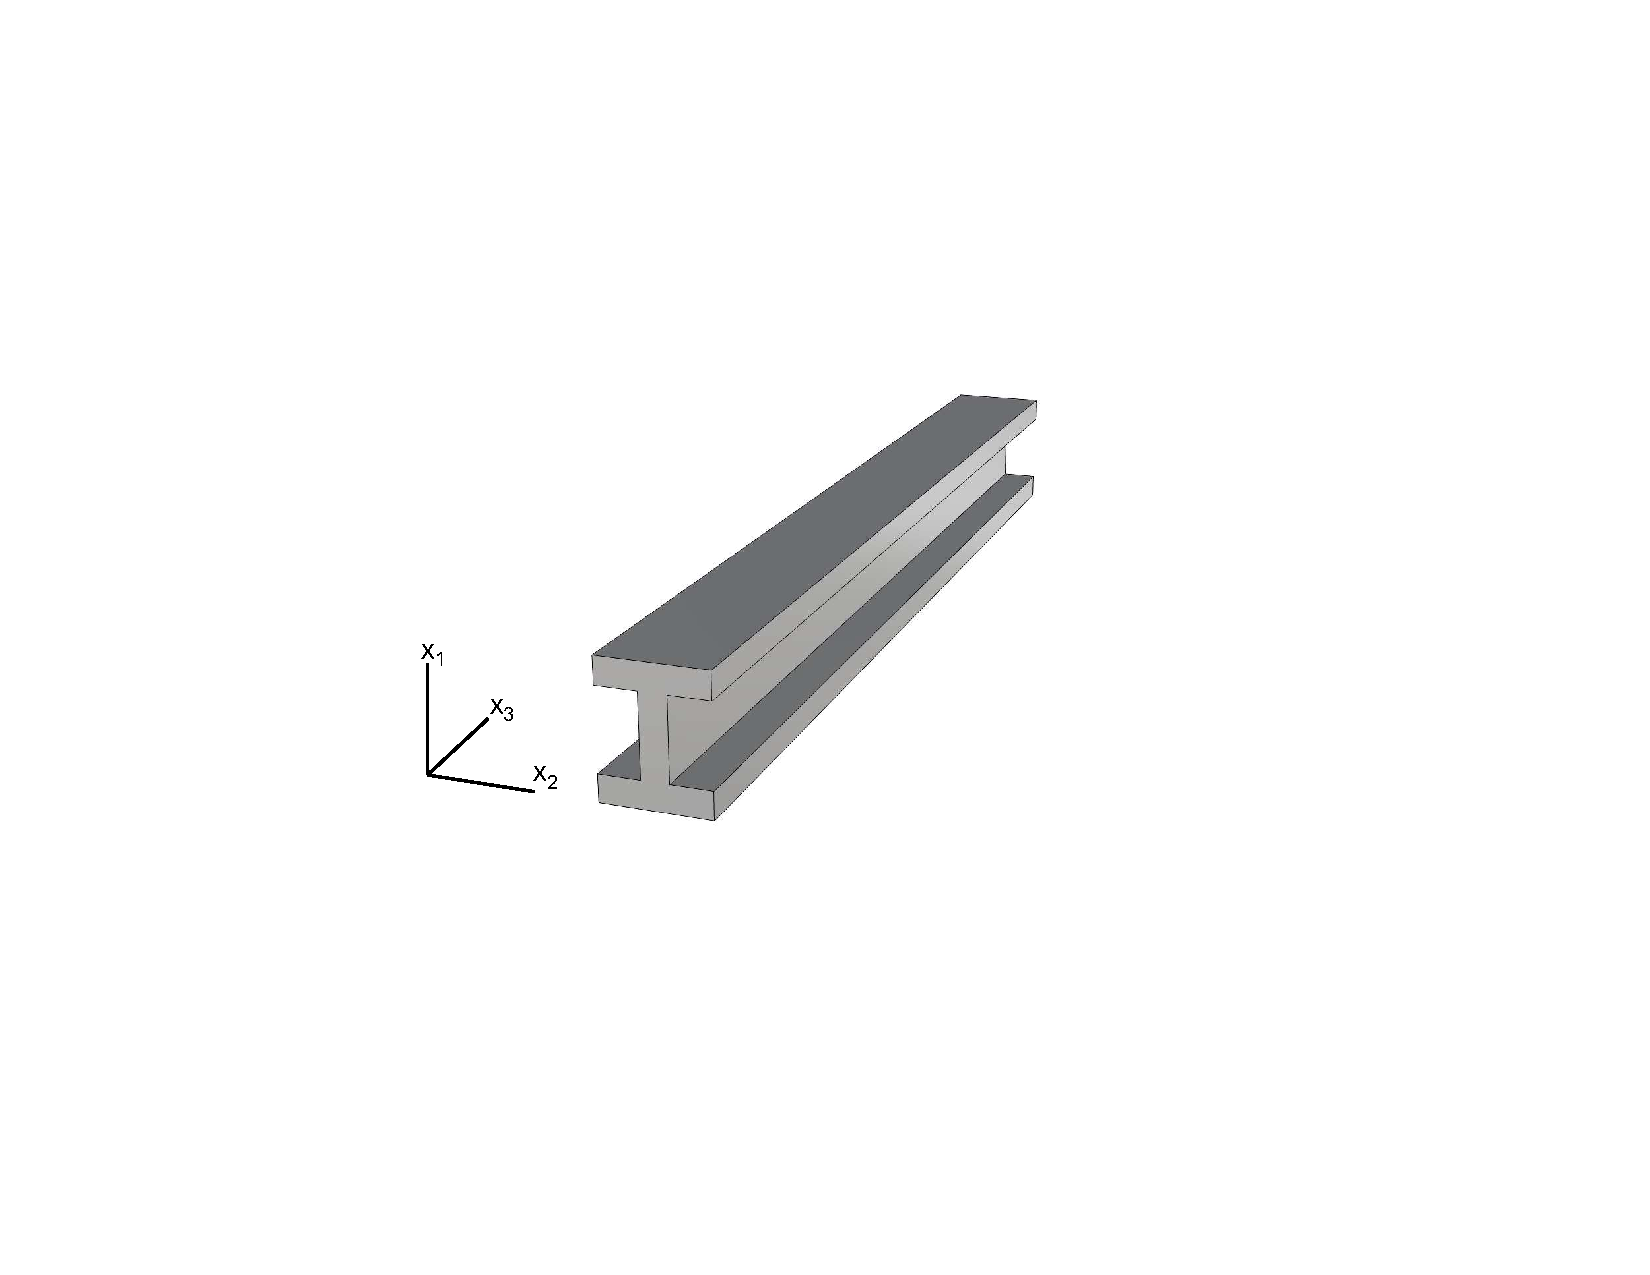
\includegraphics[width=0.2\columnwidth,trim=4cm 7cm 6cm 6.5cm, clip]{figs/straight.pdf}
}
\subfloat[$\theta_2$]{
	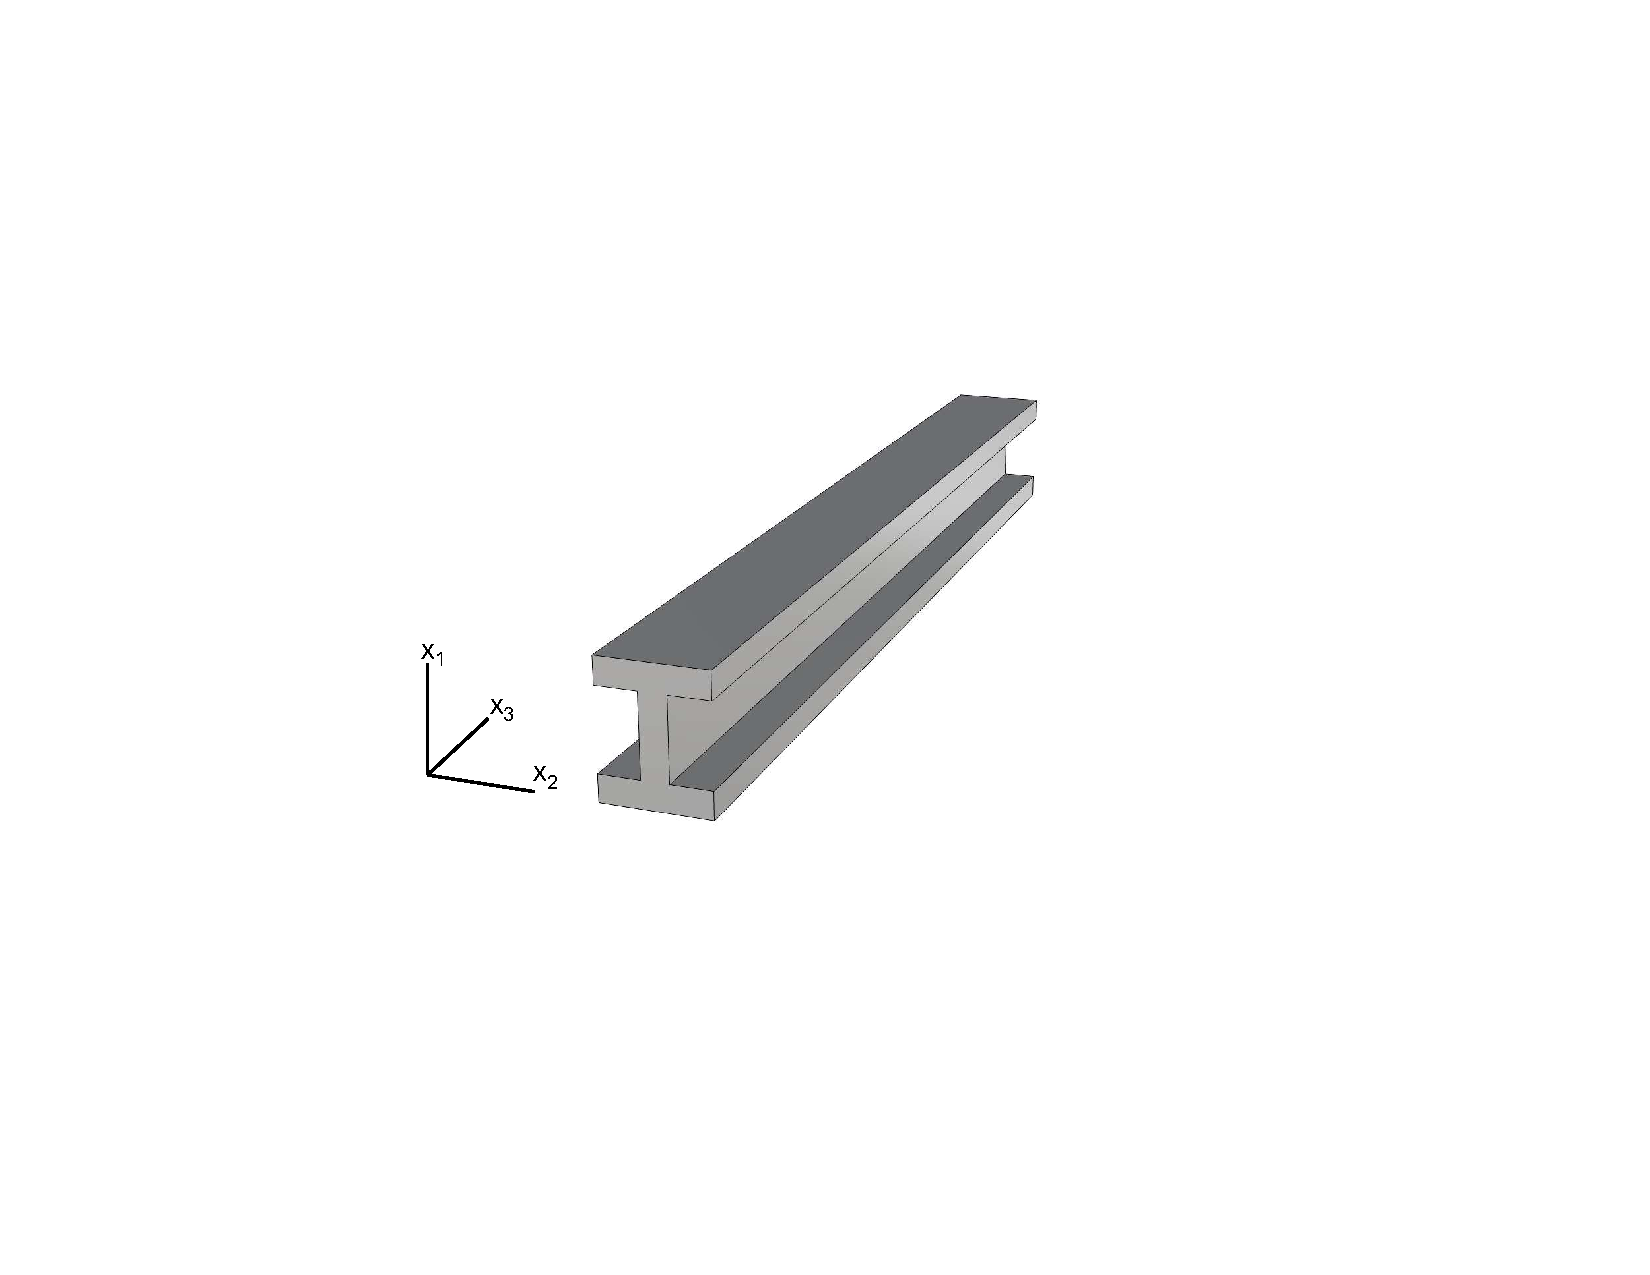
\includegraphics[width=0.2\columnwidth,trim=4cm 7cm 6cm 6.5cm, clip]{figs/straight.pdf}
}
\subfloat[$\theta_3$]{
	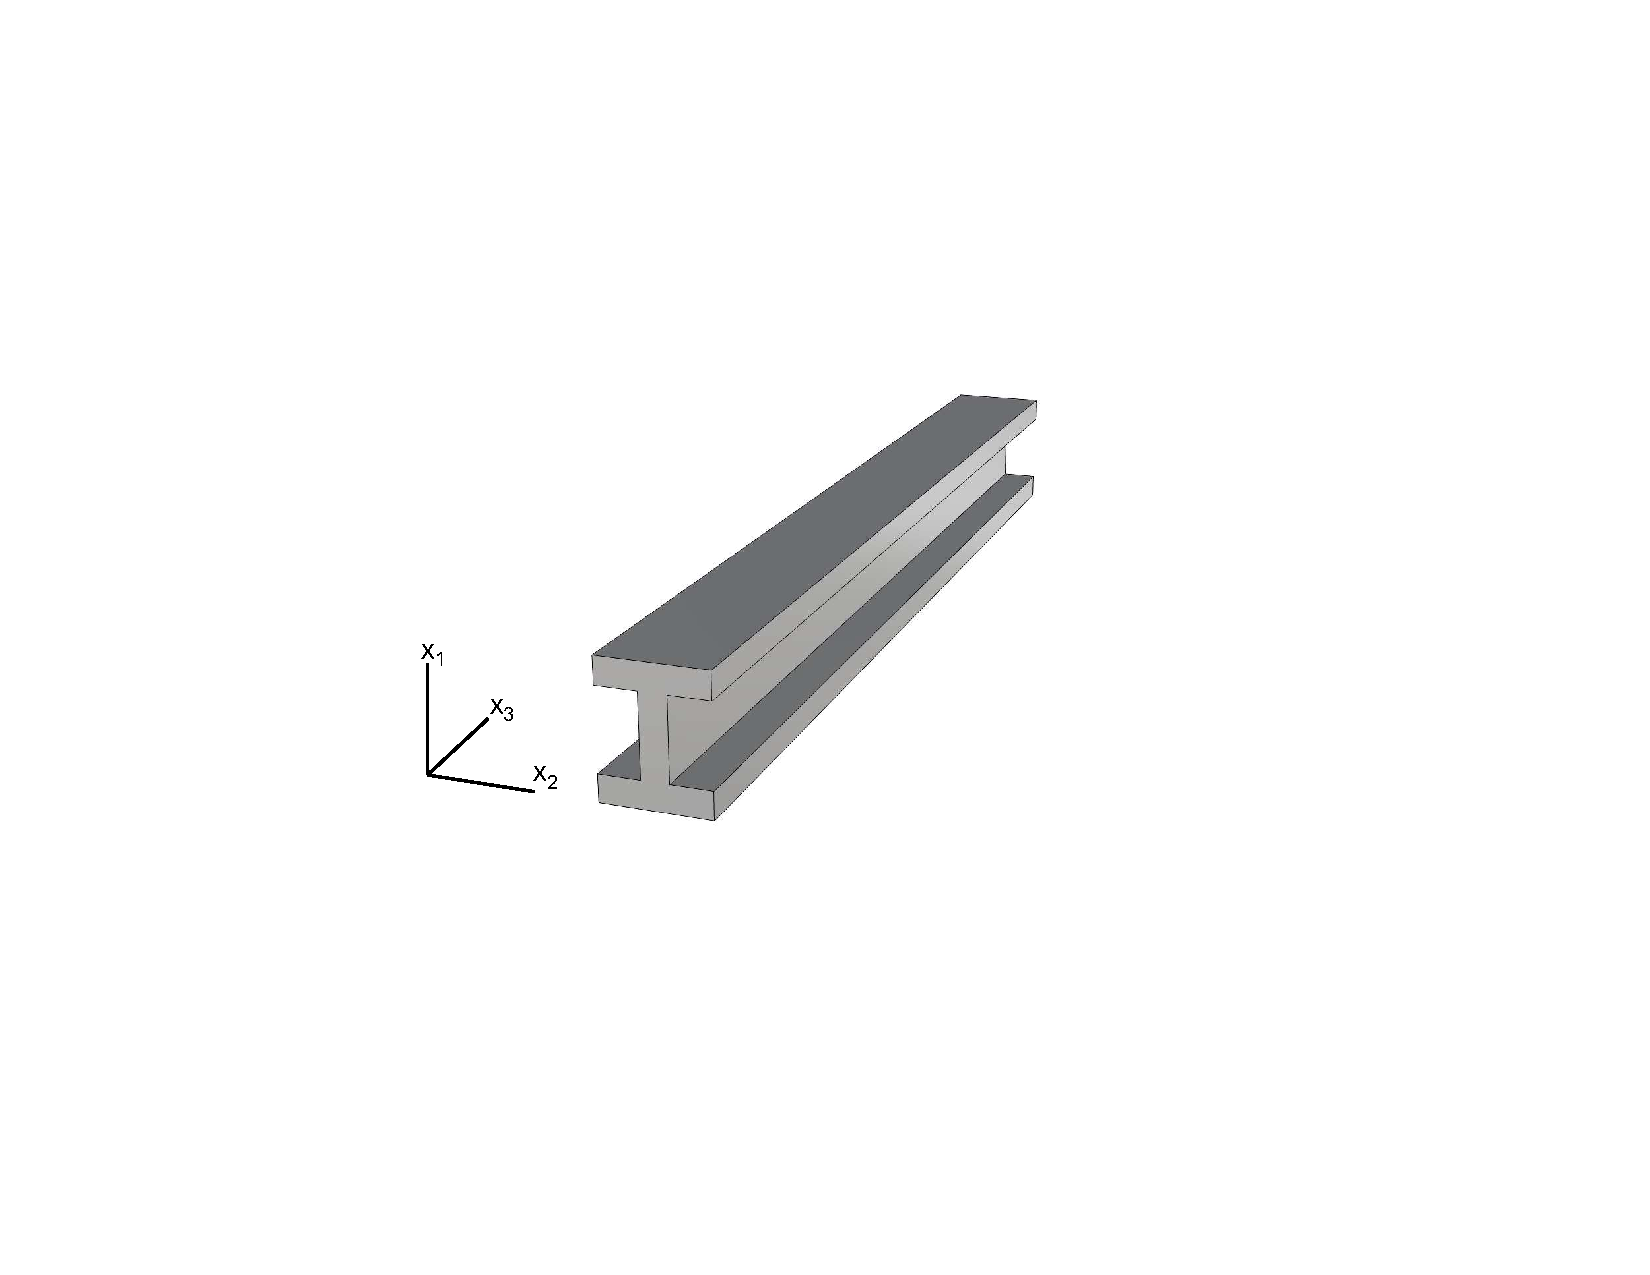
\includegraphics[width=0.2\columnwidth,trim=4cm 7cm 6cm 6.5cm, clip]{figs/straight.pdf}
}
\label{fig:w_theta_displacements}
\caption{Positive displacements in each coordinate direction for both translation and rotation are shown. CHANGE PICTURES}
\end{figure}

Note that in \cref{eq:u1} the $x_2\theta_3(x_3)$ term is subtracted $w_1(x_3)$, while in \cref{eq:u2} $x_1\theta_3(x_3)$ is added to $w_2(x_3)$.
This is an artifact of the positive/negative convection for rotation.
For a point $P$ at some positive valued $(x_1,x_2)$, the $u_1$ displacement is decreased by a $x_3$ rotation.
Similarly for the same point $P$, the $u_2$ displacement is increased by the $\theta_3$ rotation, see \cref{fig:u1u2_plus_minus_xtheta}.
The same sort of scenario occurs in \cref{eq:u3}, see \cref{fig:u3_plus_minus_xtheta}

\begin{figure}
\centering
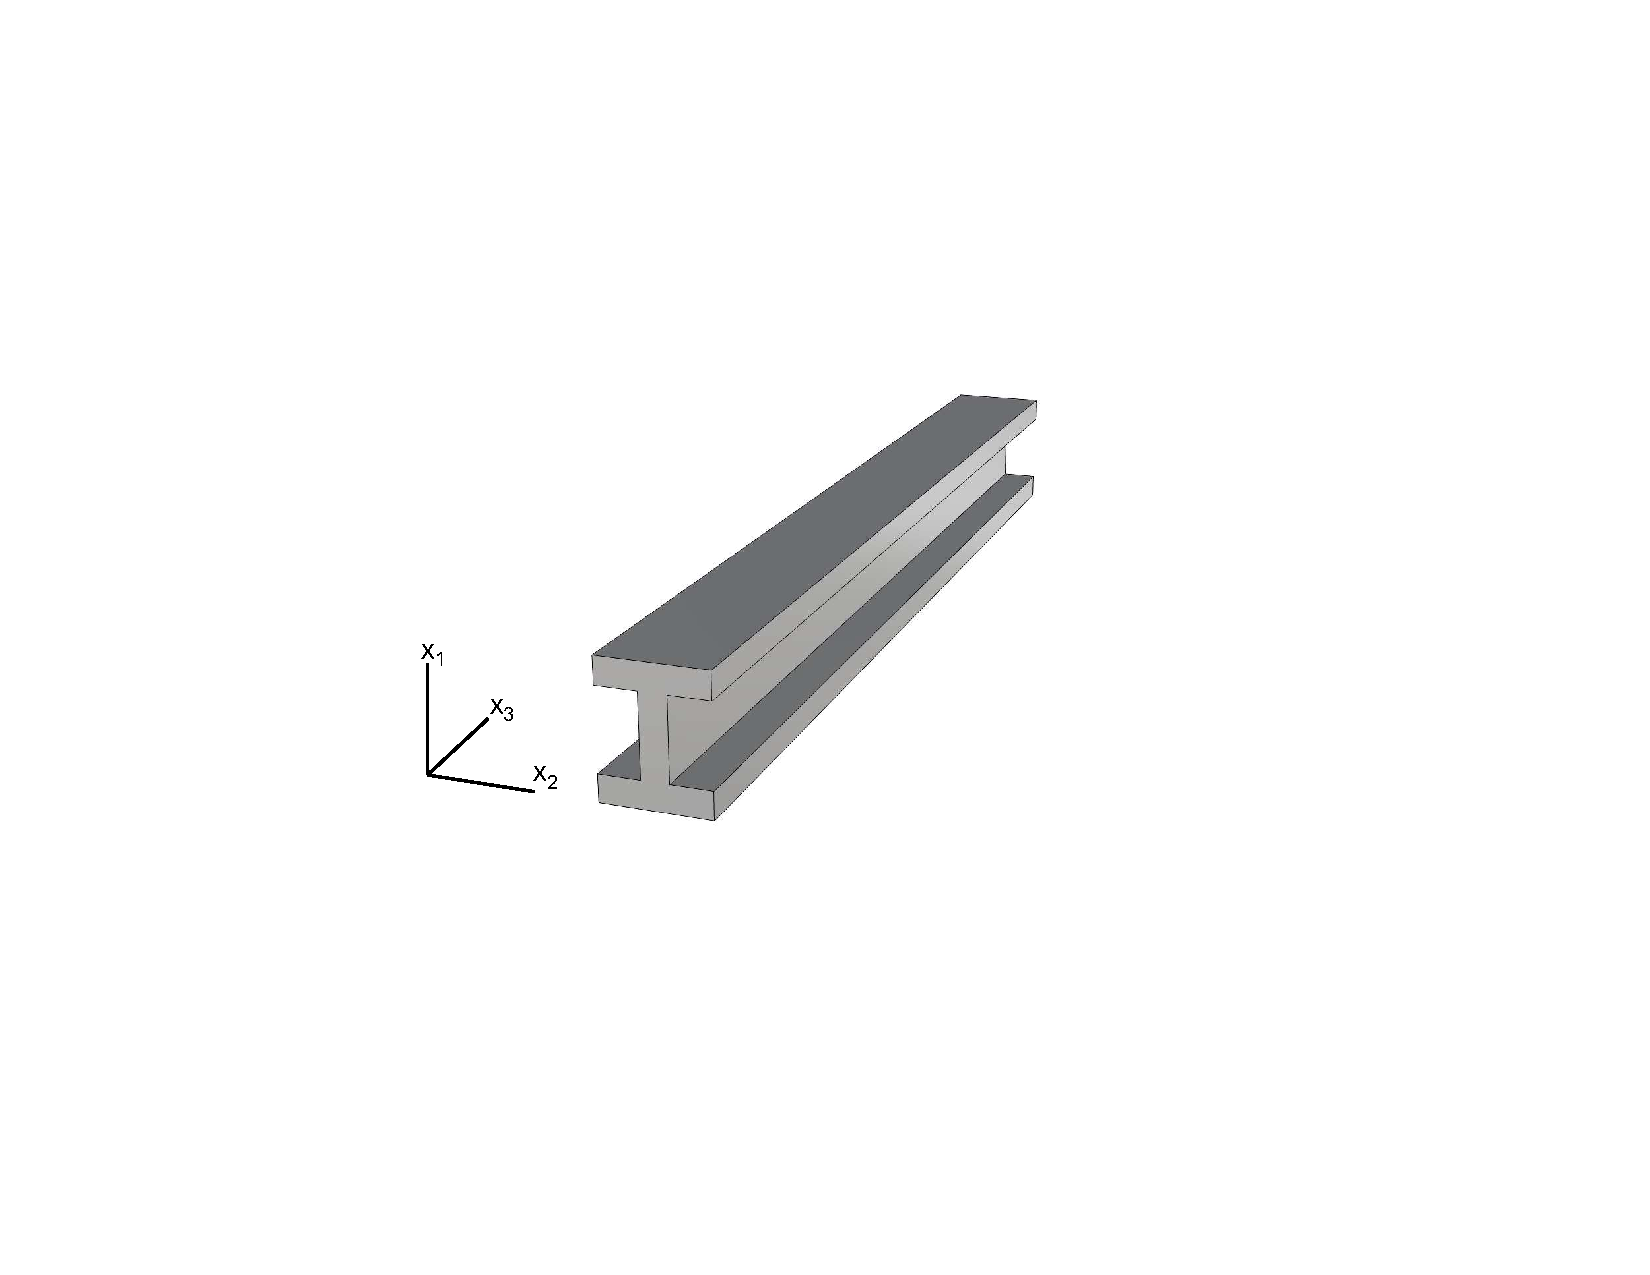
\includegraphics[width=0.2\columnwidth,trim=4cm 7cm 6cm 6.5cm, clip]{figs/straight.pdf}
\caption{A pictoral representation of sign convetion for $\theta_3$ rotations affecting $u_\alpha$ displacements. CHANGE PICTURE}
\label{fig:u1u2_plus_minus_xtheta}
\end{figure}

\begin{figure}
\centering
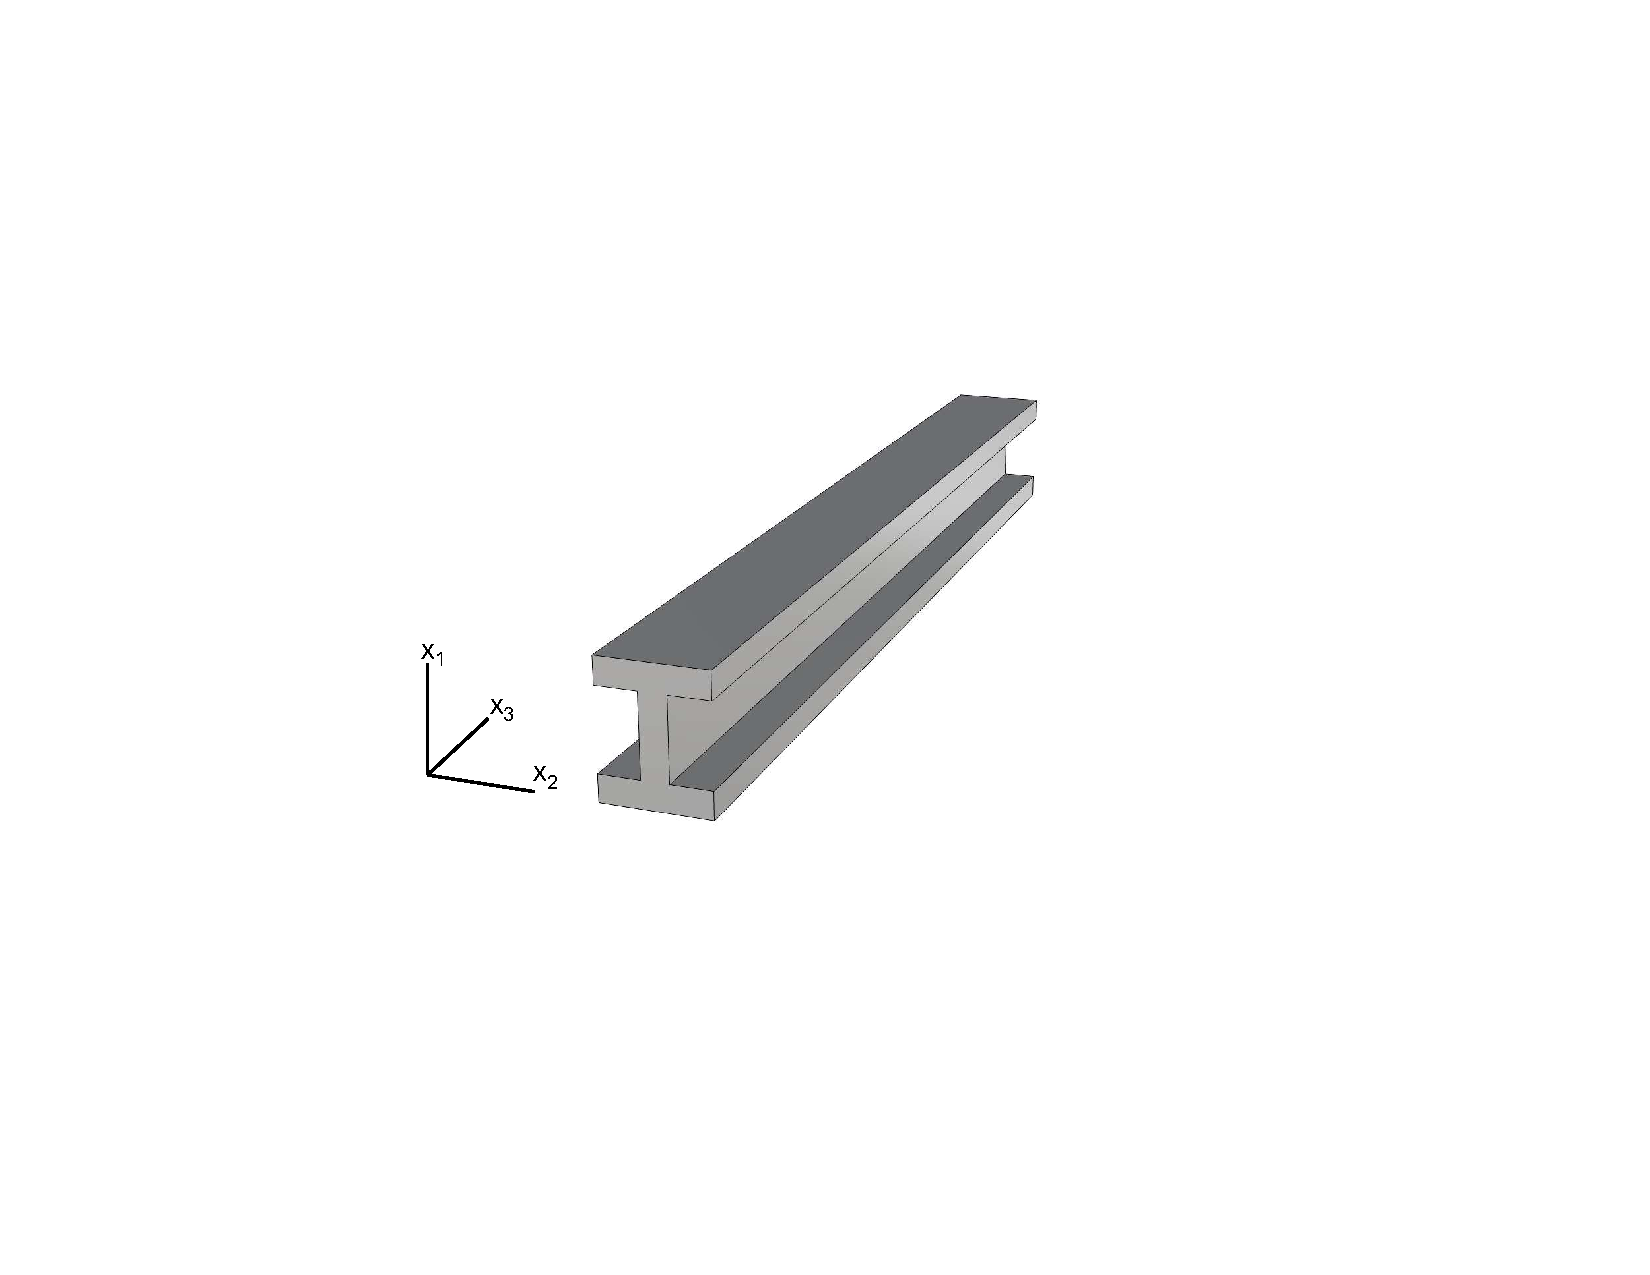
\includegraphics[width=0.2\columnwidth,trim=4cm 7cm 6cm 6.5cm, clip]{figs/straight.pdf}
\caption{A pictoral representation of sign convetion for $\theta_\alpha$ rotations affecting $u_3$ displacements. CHANGE PICTURE}
\label{fig:u3_plus_minus_xtheta}
\end{figure}

It is important to note that the anlysis will be limited or enhanced by the accuracy of these equations.
In this case, warping in the beam is not accounted for.

\section{Linear Elasticity}
\label{sec:continuum_mechanics}

Now that the beam and it's behavior are defined by the above assumptions, it is time to introduce linear elasticity.
%\Cref{eq:linear_momentum,eq:hookes_law,eq:strain,eq:displacements,eq:forces} are the equations used to describe linear elasticity.

Recall that \cref{eq:linear_momentum} represents the balance of linear momentum. 

\begin{equation}
\sigma_{ij,j} 
+
f_i 
= 
\rho 
u_{,tt}
\label{eq:linear_momentum}
\end{equation}

For static cases, it is accurate to assume that $u_{,tt} = 0$.
This assumption allows for the simplification to \cref{eq:linear_momentum_zero}

\begin{equation}
\sigma_{ij,j}+f_i = 0
\label{eq:linear_momentum_zero}
\end{equation}

\Cref{eq:hookes_law} is commonly known as hooke's law.
It relates stress and strain using the fourth order tensor $C_{ijkl}$.

\begin{equation}
\sigma_{ij} = C_{ijkl}\epsilon_{kk}
\label{eq:hookes_law}
\end{equation}

As mentioned ealier, in this work we make the assumption that the beam consists of a homogenous and isotropic material.
Therefore, Hooke's law takes the special form of \cref{eq:special_hookes}.
%, where $\lambda$ and $\mu$ are Lame\'e constants describing material properties.

The infinitesimal strain tensor is described in \cref{eq:infinitesimal_strain}.

\begin{equation}
\epsilon_{ij}=\frac{1}{2}(u_{i,j}+u_{j,i})
\label{eq:infinitesimal_strain}
\end{equation}

This is often written as \cref{eq:strain} for simplifyed notation.

\begin{equation}
\epsilon_{ij}=u_{(i,j)}
\label{eq:strain}
\end{equation}

When performing a linear elastic analysis, the quantities of interest are typically forces and displacemnts.
To solve for the unkonw forces and displacements, we begin with those that are known. 
\Cref{eq:displacements} describe the known displacements, typically  at the boundary conditions.
\Cref{eq:forces} are the known forces acting on the beam.

\begin{equation}
u_i=g_i \ on \ \Gamma_g
\label{eq:displacements}
\end{equation}

\begin{equation}
\sigma_{ij}n_j=h_i \ on \ \Gamma_h
\label{eq:forces}
\end{equation}

With the theory of linear elasticity defined, it is now possible to address the calculation of $\epsilon_{\alpha\beta}$.
By the assumptions of \cref{subsec:displacements}, we find that $\epsilon_{\alpha\beta} = 0$.
This is shown by recalling th displacement vector $u_i$ and \cref{eq:strain}.
Solving for $u_{\alpha,\beta}$ yeilds \cref{eq:grad_u}.

\begin{equation}
u_{\alpha, \beta} =
\begin{bmatrix}
 0 \ -\theta_3(x_3)\\
 \theta_3(x_3) \ 0
\end{bmatrix}
\label{eq:grad_u}
\end{equation}

Expanding $\epsilon_{\alpha\beta}$ yeilds \cref{eq:eps_alpha_beta_zero}.

\begin{align}
\label{eq:eps_alpha_beta_zero}
\epsilon_{\alpha\beta} &=\frac{1}{2}(u_{1,2}+u_{2,1}) \\
&=\frac{1}{2}(-\theta_3(x_3)+\theta_3(x_3)) \nonumber \\
&=0 \nonumber
\end{align}

Thus we verify that according to our assumptions of \cref{subsec:displacements} $\epsilon_{\alpha\beta} = 0$.
However, we will use \cref{eq:eps_alpha_beta} to calculate the strain for $\alpha$ and $\beta$ directions.

\begin{equation}
\epsilon_{\alpha \beta} = -\frac{\lambda\epsilon_{33}}{2(\lambda + \mu)}\delta_{\alpha\beta}
\label{eq:eps_alpha_beta}
\end{equation}

This equation is derived from the assumptions in \cref{subsec:stress_tensor}, which can be used to redifine $\sigma_{\alpha \beta}$ as \cref{eq:special_sigma_alpha_beta}.
This in turn expands to \cref{eq:expanded_hookes}.

\begin{equation}
0 =\sigma_{\alpha\beta} =\lambda\delta_{\alpha\beta}\epsilon_{kk}+2\mu\epsilon_{\alpha\beta}
\label{eq:special_sigma_alpha_beta}
\end{equation}

\begin{align}
\label{eq:expanded_hookes}
0 = \sigma_{\alpha\alpha} = \lambda(\epsilon_{11}+\epsilon_{22}+\epsilon_{33})\delta_{11}+2\mu\epsilon_{11}\\
+ \lambda(\epsilon_{11}+\epsilon_{22}+\epsilon_{33})\delta_{22}+2\mu\epsilon_{22} \nonumber
\end{align}

Finally, simplifying we obtain \cref{eq:eps_alpha_alpha}.

\begin{align}
0 &=\lambda(2\epsilon_{\alpha\alpha} + 2\epsilon_{33})+2\mu\epsilon_{\alpha\alpha} \nonumber \\
\epsilon_{\alpha\alpha} &= -\frac{\lambda}{\lambda+\mu}\epsilon_{33}
\label{eq:eps_alpha_alpha}
\end{align}

From here, \cref{eq:eps_alpha_beta} can be found by substituting the previous equation into \cref{eq:special_sigma_alpha_beta}. 

It has been shown that the assumptions of \cref{subsec:stress_tensor,subsec:displacements} are inconsistent with repsect to strain, in particular $\epsilon_{\alpha\beta}$.
Typically, \cref{eq:eps_alpha_beta} is prefered for strain calculations.
Also, this inconsistenty does not void the analysis method.
%Rather, it is rationalized by it's usefulness~\cref{hughes-fem}.
\section{Variational Equation}
The variational equation (a.k.a virtual work) is the next step towards FEM.
It is shown in~\cref{eq:virtual_work}.

\begin{equation}
\int_{\Omega} \sigma_{ij,j} \, \hat{u}_i \, d\Omega 
+ \int_{\Omega} f_i \, \hat{u}_i \, d\Omega 
= 0
\label{eq:virtual_work}
\end{equation}

By applying the divergence theorem, boundary conditions, and changes of variables, we arrive at~\cref{eq:fem}.

\begin{equation}
0 = \sum_{e=1}^{n_{el}} \int_{0}^{l^e} 
\left(
\hat{u}_1 \bar{u}_1 \ddot{u}_1 + 
\hat{u}_2 \bar{u}_2 \ddot{u}_2 + 
\hat{u}_3 \bar{u}_3 \ddot{u}_3 + 
\hat{\theta}_x \bar{I}_x \ddot{\theta}_x + 
\hat{\theta}_y \bar{I}_y \ddot{\theta}_y + 
\hat{\theta}_z \bar{I}_z \ddot{\theta}_z
\right) d\xi
\label{eq:fem}
\end{equation}

This is the discretized weak form of the virtual work equation, which is used for FEM formulation.
Essentially, this is the boundary between continuum mechanics and FEM.
To continue into FEM basis functions are applied, and the equations are implemented in a matrix formulation.
To continue to derive FEM for a Timoshenko beam refer to~\cite{hughes-fem}.
\section{Time Spent}
I spent 37 hours on my final project.

%\input{sections/abstract}
%
%% Introduction Section
%\section{Introduction}

The purpose of this project is to make a clear connection between the fields of continuum mechanics and the finite element method. 
The material presented herein is based on Hughes chpt 5.4 and Dr. Shepherd's Timoshenko Frame Derivation.
The motivation for undertaking this project is first and foremost to help myself gain a better understanding of these topics. 
I also hope that my work here will also help to accelerate other students learning as they try to understand the connection between continuum mechanics and the finite element method. 

{\Rd make this different, more like a real paper}
I think it would be helpful to say $\alpha$ and $\beta$ (greek) represent 1 and 2 while $e$ and $i$ (latin) represent 1, 2, and 3
%
%\input{sections/background_material}
%
%\input{sections/methodology}
%
%\input{sections/results}
%
%\input{sections/conclusion}

% references don't count against the 4 page limit
\newpage 

%\section*{Acknowledgements}
%\input{sections/ack.tex}
%\input{sections/sandia-disclaimer.tex}
\newpage

%% if using BibTex
\bibliographystyle{siam}
\bibliography{references}

\end{document}
